\renewcommand{\arraystretch}{1.2}
\section{Analysis}
In this section, we present the analysis of the obtained data. The structure of the analysis is as follows: We start 
of with analyzing the monochromator. To this end, we investigate its calibration with the Hg-lamp's peaks, examine 
the influence of the slit width, identify the upper boundary of detection (in terms of wavelength) and measure the 
different detection probabilities for vertically and horizontally polarized light. 
Then we visualize the measured spectrum overviews of three samples, carbon disulfide (CS$_2$), chloroform (CHCl$_3$),
and carbon tetrachloride (CCl$_4$) and identify visible Stokes 
and Anti-Stokes peaks. The data is of rather bad quality, having a low signal-to-noise ratio. Especially under the given 
time constraints, we were not able to obtain better signals by adjusting the accessible experimental parameters. We 
therefore have to refrain from doing further analysis with these spectra. 

Instead, we decided to do the bulk of the analysis on data taken by the CCD spectrometer. The corresponding second part 
of the analysis follows a similar structure. We start of by verifying the calibration of the CCD spectrometer with the 
Hg-lamp, continued by the sensitivity analysis regarding polarized light with a resulting correction factor. Proceeding 
differently to the prior analysis, we go on by investigating the laser used in the experiment. Then we examine the 
properties of the notch filter used in all of the spectra later on. This is done in a qualitative manner since there was 
no possibility of changing the parameters of this part of the experiment. 

The most important part of the analysis comes at this point: The analysis of the spectra of all samples at hand. For 
the first two, CS$_2$, CHCl$_3$, we only fit all visible peaks and compare the results to literature values. The following 
samples, however, are each used to highlight as specific aspect connected to Raman spectroscopy. The CCl$_4$ sample is 
used to demonstrate the effects of asymmetry in the molecule, resulting in a depolarization of the scattered light. The 
linear dependence of the intensity of Raman peaks on the concentration of the corresponding substance is used to measure 
the concentration of ethanol in an unknown ethanol-water mixture, highlighting a widely used application of Raman 
spectroscopy for characterizing unknown substances. And a final analysis of a measurement of sulfur is used to measure the 
temperature of the probe. Although of questionable reliability, this last part demonstrates the theoretical connection 
between the experiment and results of statistical mechanics. 

The literature values in this section, namely the wavenumbers of various peaks, are taken from the NIST 
Computational Chemistry Comparison and Benchmark DataBase\cite{nist}.
\subsection{Techniques used for the evaluation}
All calculations in this section are done with scripts written in 
the \textit{python} programming language~\cite{python}, relaying in several 
packages:
\begin{itemize}
    \item
        \textit{matplotlib}~\cite{Hunter2007} for plotting,
    \item
        \textit{scipy}~\cite{scipy} for fitting, and 
    \item
        \textit{uncertainties}~\cite{uc} for error propagation.
\end{itemize}
The latter applies Gaussian error propagation for correlated and uncorrelated variables. 
We will thus not explicitly write down the formulas for the error propagation 
for each quantity calculated but instead state the numerical result, only. 
We will, however make a quick remark on the use of covariance matrices in 
error propagation: Contrary to measured data, which in our case is usually 
expected to be uncorrelated, all fitted data yields variables that in general correlate. 
The propagation is then done as follows:
Let's assume we have random
variables $x_0,...,x_N$ which are correlated through the $N\times N$ Matrix $cov(x_i,x_j)$.
For a scalar function $f(x_0,...,x_N) \rightarrow \mathbb{R}$, the variance is estimated (linearly) by:
\begin{equation}
Var[f] = \sigma^2 = \sum_{i,j} \frac{\partial f}{\partial x_i} \frac{\partial f}{\partial x_j} cov(x_i,x_j) \,.
\end{equation} 
If instead, $\mathbf{f}$ is a vector field in $m$ dimensions, namely 
$\mathbf{f}(x_0,...,x_N) \rightarrow \mathbb{R}^m$, then the components of $\mathbf{f}$ 
are further correlated. We can write down the relation between the covariance matrices $V$ and $U$ of 
$\mathbf{x}$ and $\mathbf{f}$, respectively, in matrix relations:
\begin{equation}
    U = A V A^T
\end{equation}
where $A$ is the matrix defined by 
\begin{equation}
    A_{ij} = \left[ \frac{\partial f_i}{\partial x_j}\right]_{\mathbf{x} = \mu}
\end{equation}
with expectation value $E[\mathbf{x}] = \mu$.~\cite{cowan1998statistical}
In order to facilitate notation, the covariance matrices will in general be notated without 
specifying the units. If not specified explicitly, the units will correspond to those of the
variables: If $x_i, x_j$ have the units $[x_i], [x_j]$, respectively, 
then the entry of the covariance matrix has the unit $[x_i] \cdot [x_j]$. \\
\paragraph{\textbf{Important note:}}
\label{par:important note}
We will neither give the correlation matrix nor the $\chi^2/\mathrm{dof}$ in the analysis, 
because we don't consider this information crucial to our calculations. The correlated parameters will
not be combined in any of the following calculations and standard deviations are stated for all
calculated quantities. 



\clearpage


\subsection{Monochromator}
The data taken with the monochromator is closely connected to the experimental setup. Many parameters were accessible 
experimentally and had to be tuned in order to get reasonable results. We will not use all measurements taken, but only 
rely on those with the most usable results. In general, the resolution of the data is restricted by the program used for 
the recordings: Data points are separated by 0.1 nm, regardless of scanning speeds (which could be lowered down to 0.05 
nm / s). This makes fitting impossible in all cases, even in absence of noise (as for the Hg-lamps spectrum). We thus 
identify peaks by searching for local maxima in manually specified regions. The error is estimated rather generously with 
0.2 nm, twice the resolution. One has to keep in mind another source of error, namely the problem of getting the correct 
starting point for a measurement: The registration of data from the monochromator starts once the counter is moving.
However, the starting point has to be set separately for the computer and the device, inducing a possible error of ca. 
0.1 nm for each measurement. 

\subsubsection{Calibration}
The Hg-lamp's spectrum was measured with a scan speed of 2~\AA/s with a slit width of 50 $\mu$m over a range from 400 to 
600 nm. The result is plotted in figure \ref{fig:mono_calibration_hg}. The six observable peaks are found in the
literature -- a comparison is shown in table \ref{tab:mono_calibration}. Due to the good agreement, we go without a linear 
fit and use the values for the wavelength given in the original data in the following analysis. The error induced is 
negligible in comparison to the resolution and offset possibly induced each time. 
\begin{table}[htpb]
    \centering
    \caption{
        Peaks of Hg-spectrum. Notice the good agreement. 
        }
    \label{tab:mono_calibration}
    \begin{tabular}{c r r}
        \rowcolor{LightCyan} Peak & $\lambda_\text{a} \,/\, \text{nm}$ & $\lambda_\text{lit} \,/\, \text{nm}$ \\
        \cellcolor{LightCyan}$1$ & $404.6 \pm 0.2$ & $404.7$   \\
        \cellcolor{LightCyan}$2$ & $407.7 \pm 0.2$ & $407.8$   \\
        \cellcolor{LightCyan}$3$ & $435.8 \pm 0.2$ & $435.8$   \\
        \cellcolor{LightCyan}$4$ & $546.0 \pm 0.2$ & $546.1$   \\
        \cellcolor{LightCyan}$5$ & $576.9 \pm 0.2$ & $577.1$   \\
        \cellcolor{LightCyan}$6$ & $579.1 \pm 0.2$ & $579.1$ 
    \end{tabular}
\end{table}
\begin{figure}[htpb]
    \centering
    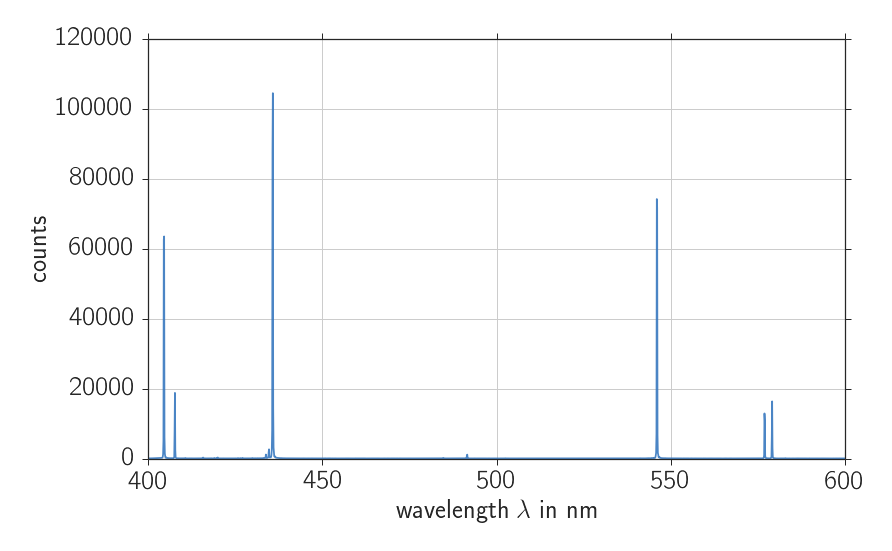
\includegraphics[width=0.8\linewidth]{analysis/figures/mono_calibration_hg}
    \caption{Spectrum of Hg-lamp recorded with the monochromator. The six visible peaks are identified and compared 
    to literature values in order to verify the calibration of the device.}
    \label{fig:mono_calibration_hg}
\end{figure}

\subsubsection{Influence of slid with}
In order to examine the effect of varying the slit width at the entrance of the monochromator, we took measurements of a 
single peak, the 404.7 nm peak of the Hg-spectrum, for width ranging from 25 to 200 $\mu$m. All measurements are taken 
with a sampling rate of 1~\AA/s. The effects are shown in 
figure \ref{fig:mono_slit}. One observed reducing intensities and widths of the peak. Further, a small effect on the 
center position of the peak is seen: For a 200 $\mu$m opening, the center of the peak is some 0.2 nm higher then for peaks 
between 150 and 40 $\mu$m. The smallest opening yields again yields a slightly higher peak center. These deviations should 
not be overinterpreted, because they might also be due to the described possible fluctuations. The yield of this analysis 
was that we stipulated the width at 100 $\mu$m for the following measurements. 

\begin{figure}[htpb]
    \centering
    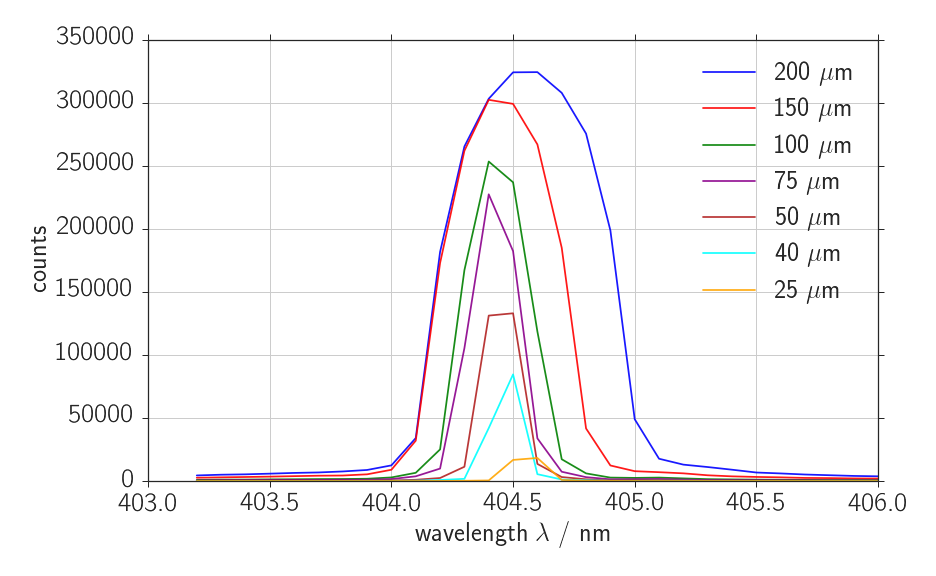
\includegraphics[width=0.8\linewidth]{analysis/figures/mono_slit}
    \caption{Effects of slit width of monochromator. Shown are various measurements of the same peak of the Hg-lamp's
    spectrum. The legend indicates the adjusted slid widths, ranging from 200 $\mu$m down to 25 $\mu$m. The effect 
    on the peaks position is well within the expected fluctuations due to difficulties in the setup. The chosen 
    width for further measurements is 100 $\mu$m. }
    \label{fig:mono_slit}
\end{figure}

\subsubsection{Boundary of detection}
The monochromator has only a limited range in which intensities at two different wavelength can be compared directly. Also 
we are not equipped to measure the invariance within the regime (one would need a light source of known intensity 
distribution), we can at least find a upper boundary in terms of wavelength. In order to do so, we assume the white light 
in the experiment to emit radiation following the intensity distribution of black-body radiation. We then compare this 
characteristic distribution with the intensity measured with the white light as the only light source. The measured counts 
at each wavelength are displayed in figure \ref{fig:mono_bound}. One clearly observes a drop in count numbers for 
wavelength above 590 nm. The drop is not abrupt but follows an exponential decay. 
However, without further quantifying the effect, one should not work with data in this regime when concerned about 
intensity. 

\begin{figure}[htpb]
    \centering
    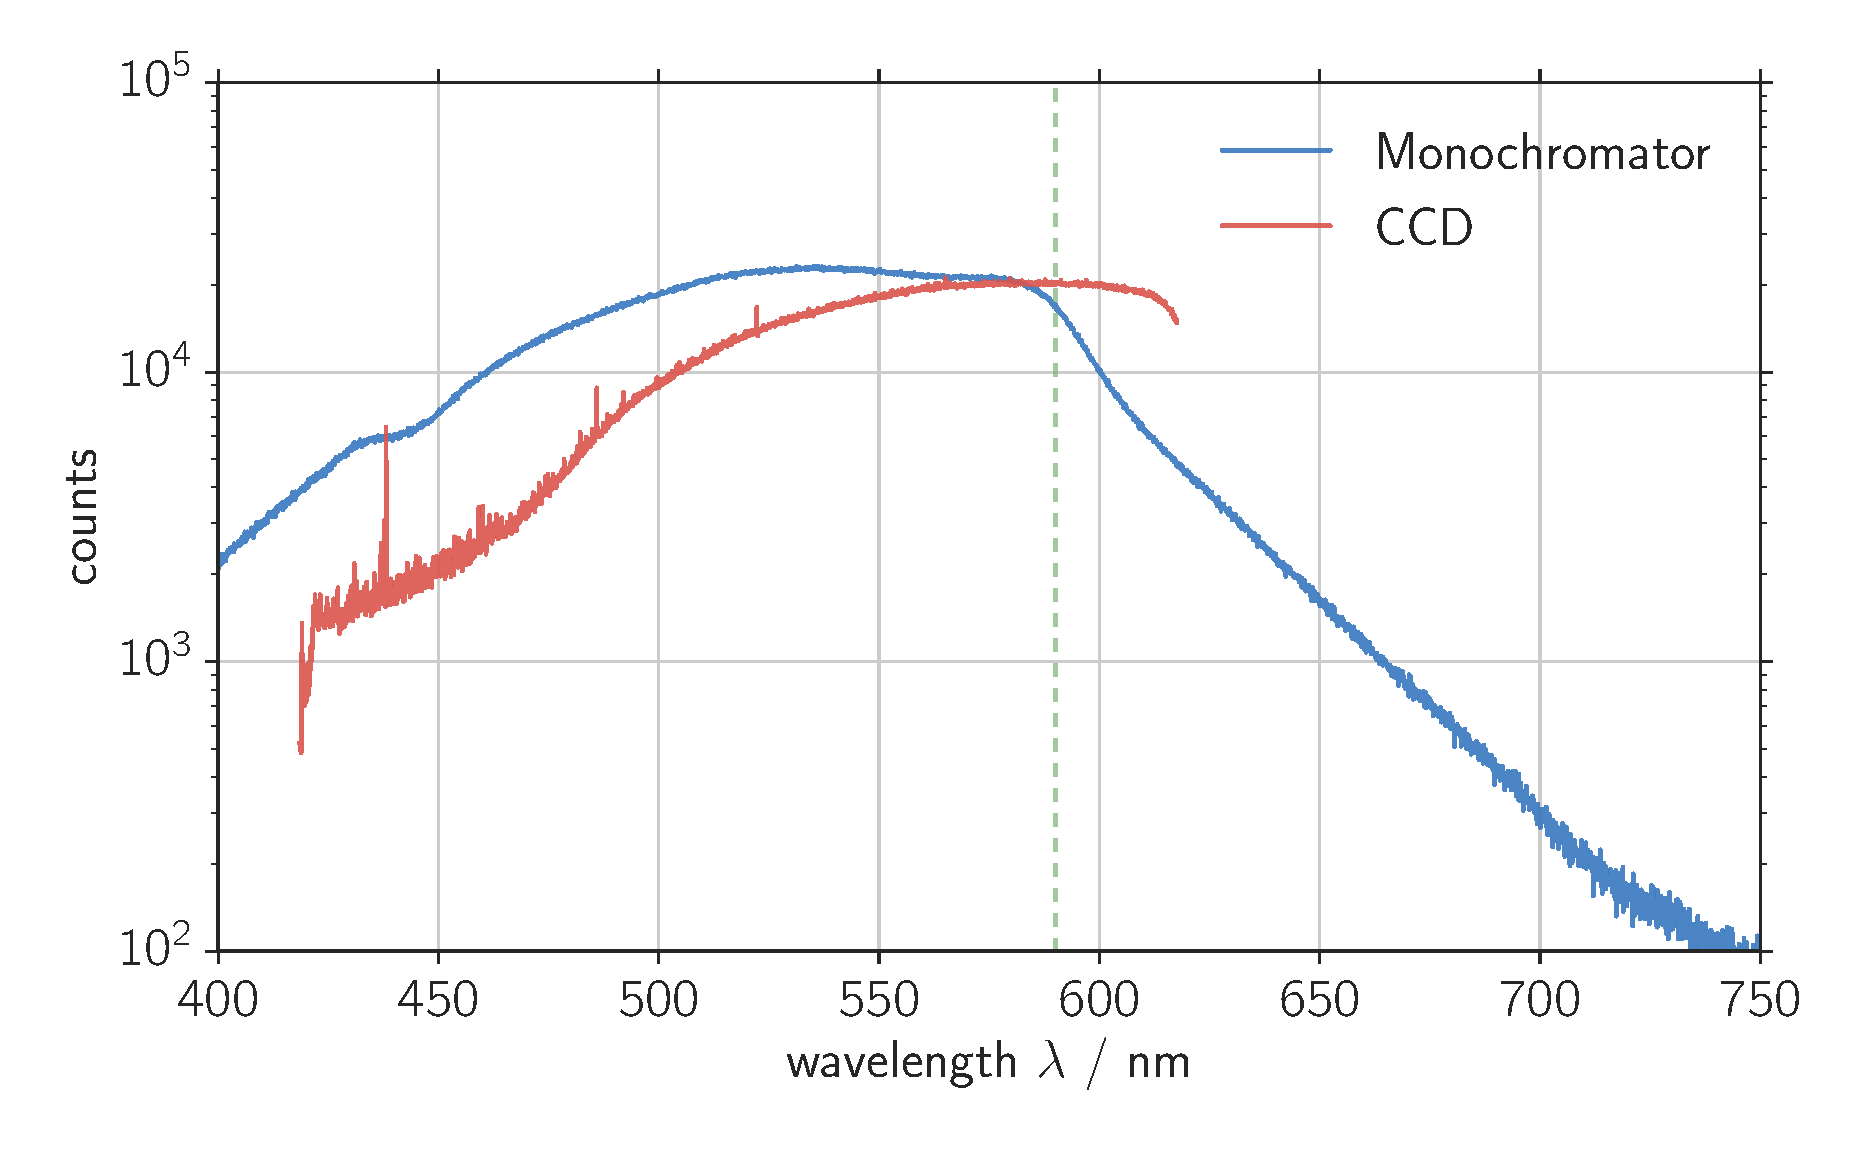
\includegraphics[width=0.8\linewidth]{analysis/figures/mono_bound}
    \caption{Spectrum of the white light on semi log scale recorded with the monochromator and the CCD spectrometer. 
        The decay in counts for wavelengths above 590 (dotted line) indicates the upper boundary of detection for the
    monochromator. The spectrum recorded with the CCD is rescaled for comparability. }
    \label{fig:mono_bound}
\end{figure}

\subsubsection{Detection probability for polarized light}  
Even though the measured spectra do not allow for a detailed analysis including the intensities of the peaks, we still 
measure the detection probability of the monochromator for light polarized vertically or horizontally. We used the white 
light, which is not polarized, and a polarization filter with the angle measured towards the vertical line. The measured
counts (see figure \ref{fig:mono_polarized}) show interesting features: First of all, the detection probability differs by 
a considerable amount for large parts of the range tested. For wavelengths below 500 nm, vertically polarized light is 
detected more easily, above 550 nm the situation is reverted. Further one can observe a step at 430 nm for horizontally 
polarized light, indicating a possible malfunction of the device. To make more precise statements, these features would 
have to be analyzed in a more rigorous manner. 

\begin{figure}[htpb]
    \centering
    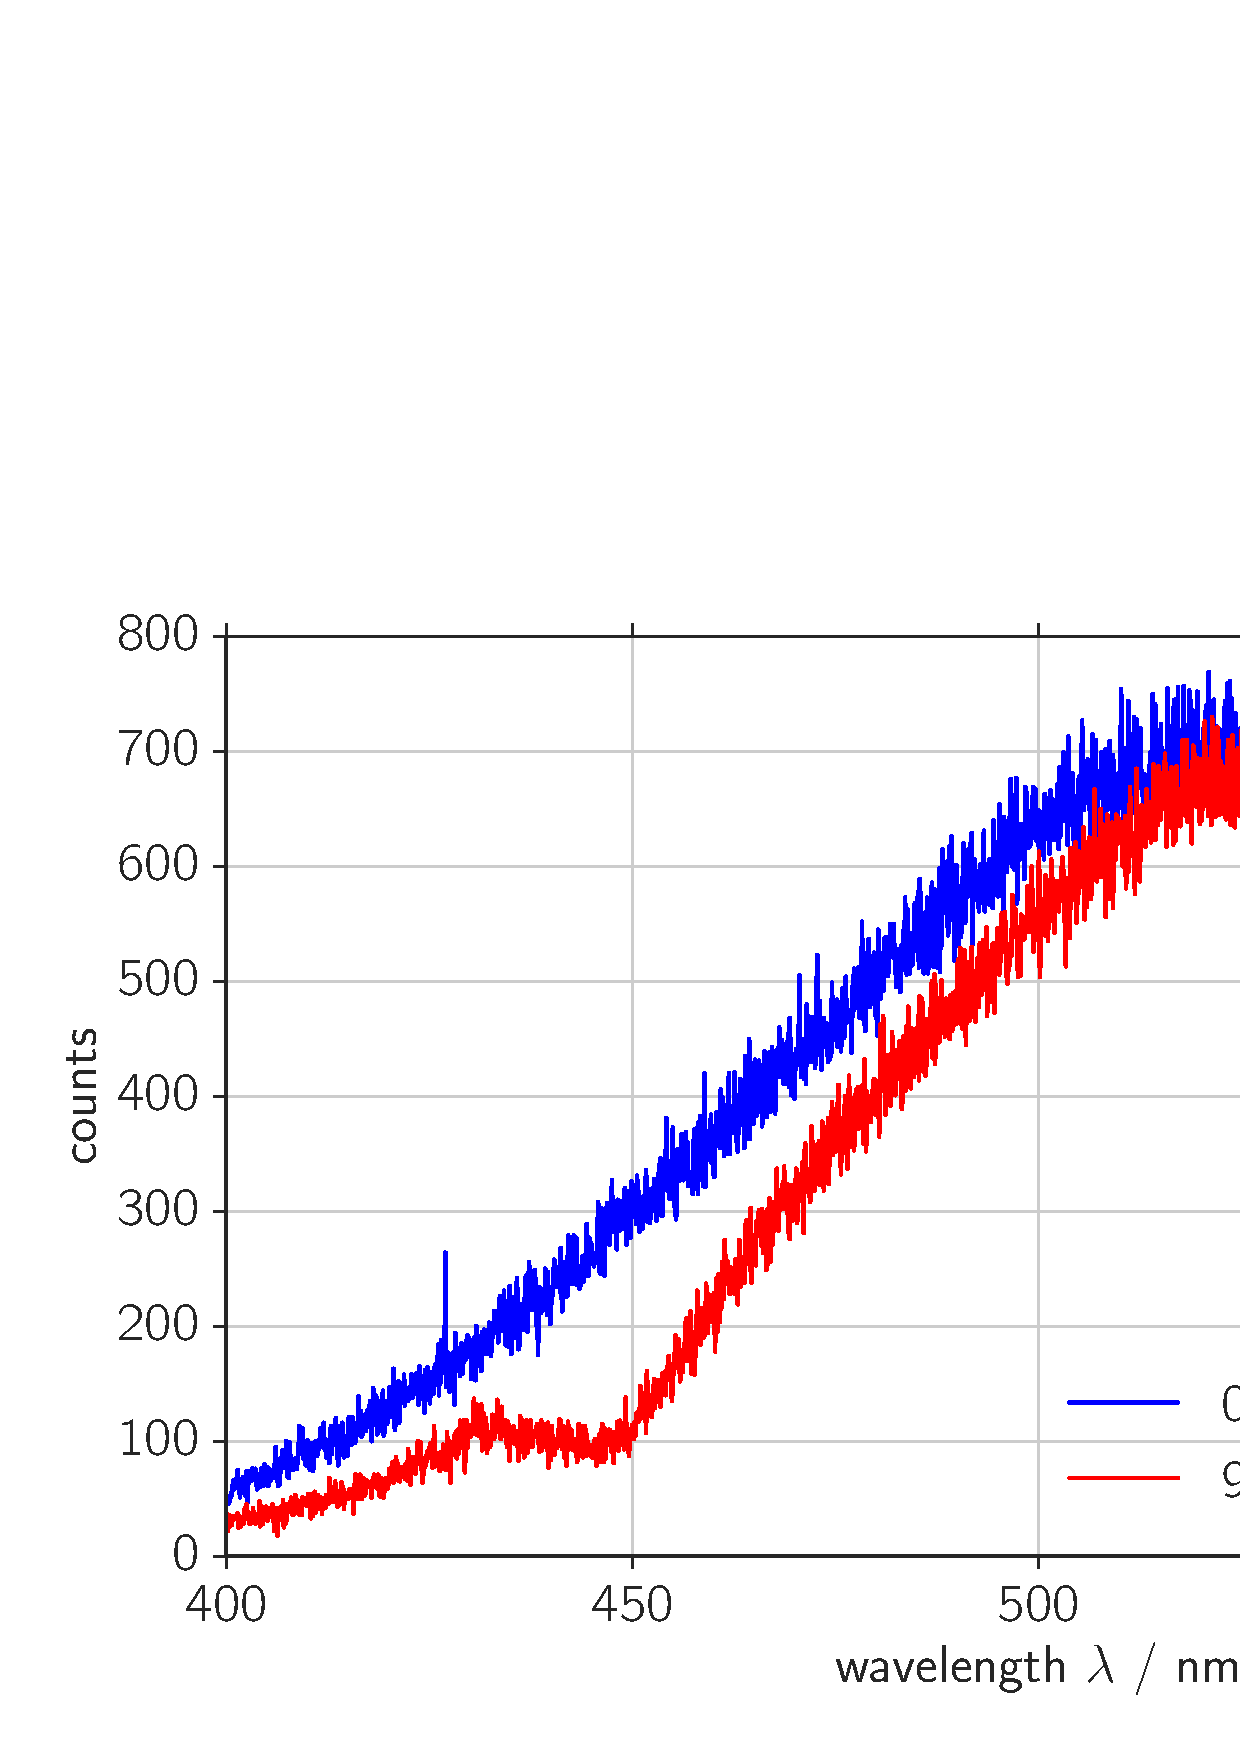
\includegraphics[width=0.8\linewidth]{analysis/figures/mono_polarized}
    \caption{Spectrum of white light with polarization filter obtained with the monochromator for two perpendicular 
    polarizations. One observes the dependency on polarization and wavelength for the detection probability. Note further 
    the step at $\lambda = 430$ nm, an unexpected feature not explained by the white light's spectrum. }
    \label{fig:mono_polarized}
\end{figure}

\subsubsection{Spectra of CS$_2$, CHCl$_3$, CCl$_4$}
The spectra of the three samples are measured under slightly varying conditions -- a remainder of our attempts to 
optimize the measurements with the monochromator. Although the original attempt (get signals usable for a quantitative 
analysis including intensity measurements) failed, we did see some peaks which are compared to the literature values in 
the following. Some parameters, however, did not change during these measurements: The slit width was left at 100 $\mu$m, 
the laser was always operated at a current of 1.5 A and we used the $\lambda / 2$ plate to turn the laser's polarization 
by $90^\circ$. Notch filter and polarization filter were not in use. 

The spectrum of carbon disulfide is shown in figure \ref{fig:mono_cs2}. We measured with a sampling speed of 
$0.05$ \AA/s and a voltage of 1000 V applied to the photomultiplier. 
The Rayleigh peak at the laser wavelength of 532 nm is not shown fully because its intensity (1.2e7 counts) 
lies two orders of magnitude above the Stokes peak's intensity.
The latter is found at $551.3 \pm 0.2$ nm, which yields a wavenumber of $653 \pm 14 \text{ cm}^{-1}$ for the respective
vibrational mode.%
\footnote{
    To calculate the wavenumber, we use a laser wavelength of $532.1 \pm 0.3$ nm, an anticipated result of the analysis
    done with the CCD, see section \ref{sec:laser}.
} The literature value of this vibrational mode is $658 \text{ cm}^{-1}$, which is covered quite well within the error.   

\begin{figure}[htpb]
    \centering
    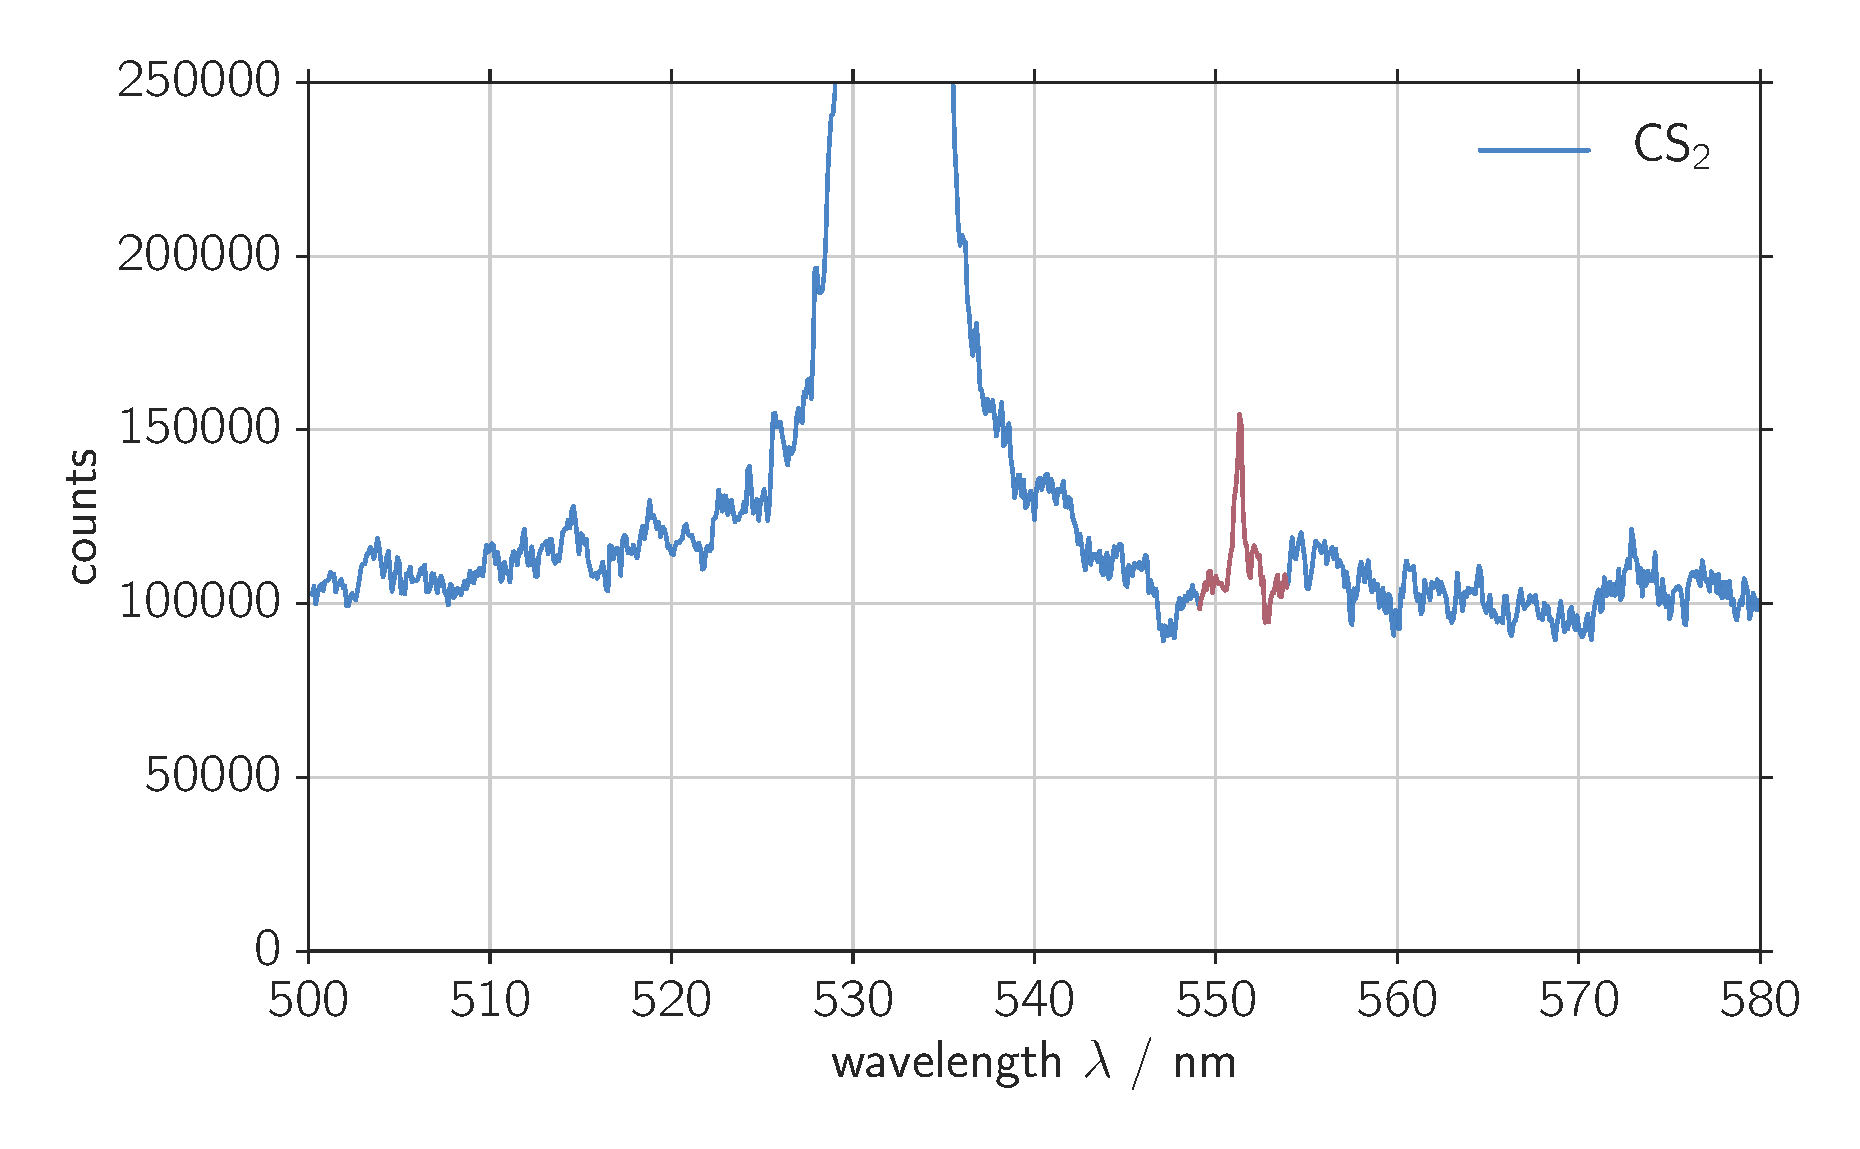
\includegraphics[width=0.8\linewidth]{analysis/figures/mono_cs2}
    \caption{Spectrum of carbon disulfide recorded with the monochromator. Only one Stokes peak is visible (highlighted).
    Background rate as well a noise are abundant. }
    \label{fig:mono_cs2}
\end{figure}


For chloroform (CHCl$_3$) we applied 1000 V to the photomultiplier and sampled with 0.1~\AA/s. The result can be seen in 
figure \ref{fig:mono_chcl3}. Three Stokes peaks are found. Their wavelength and -numbers as well as literature values are 
displayed in table \ref{tab:mono_chcl3}. Especially for the first two peaks, the agreement with the literature is good. 
The last peak is off by more than one standard deviation which shows the strong limitations on our data. Since the 
literature values lack specifications on the intensity of each peak, we cannot derive further conclusions from that
direction either. 

\begin{figure}[htpb]
    \centering
    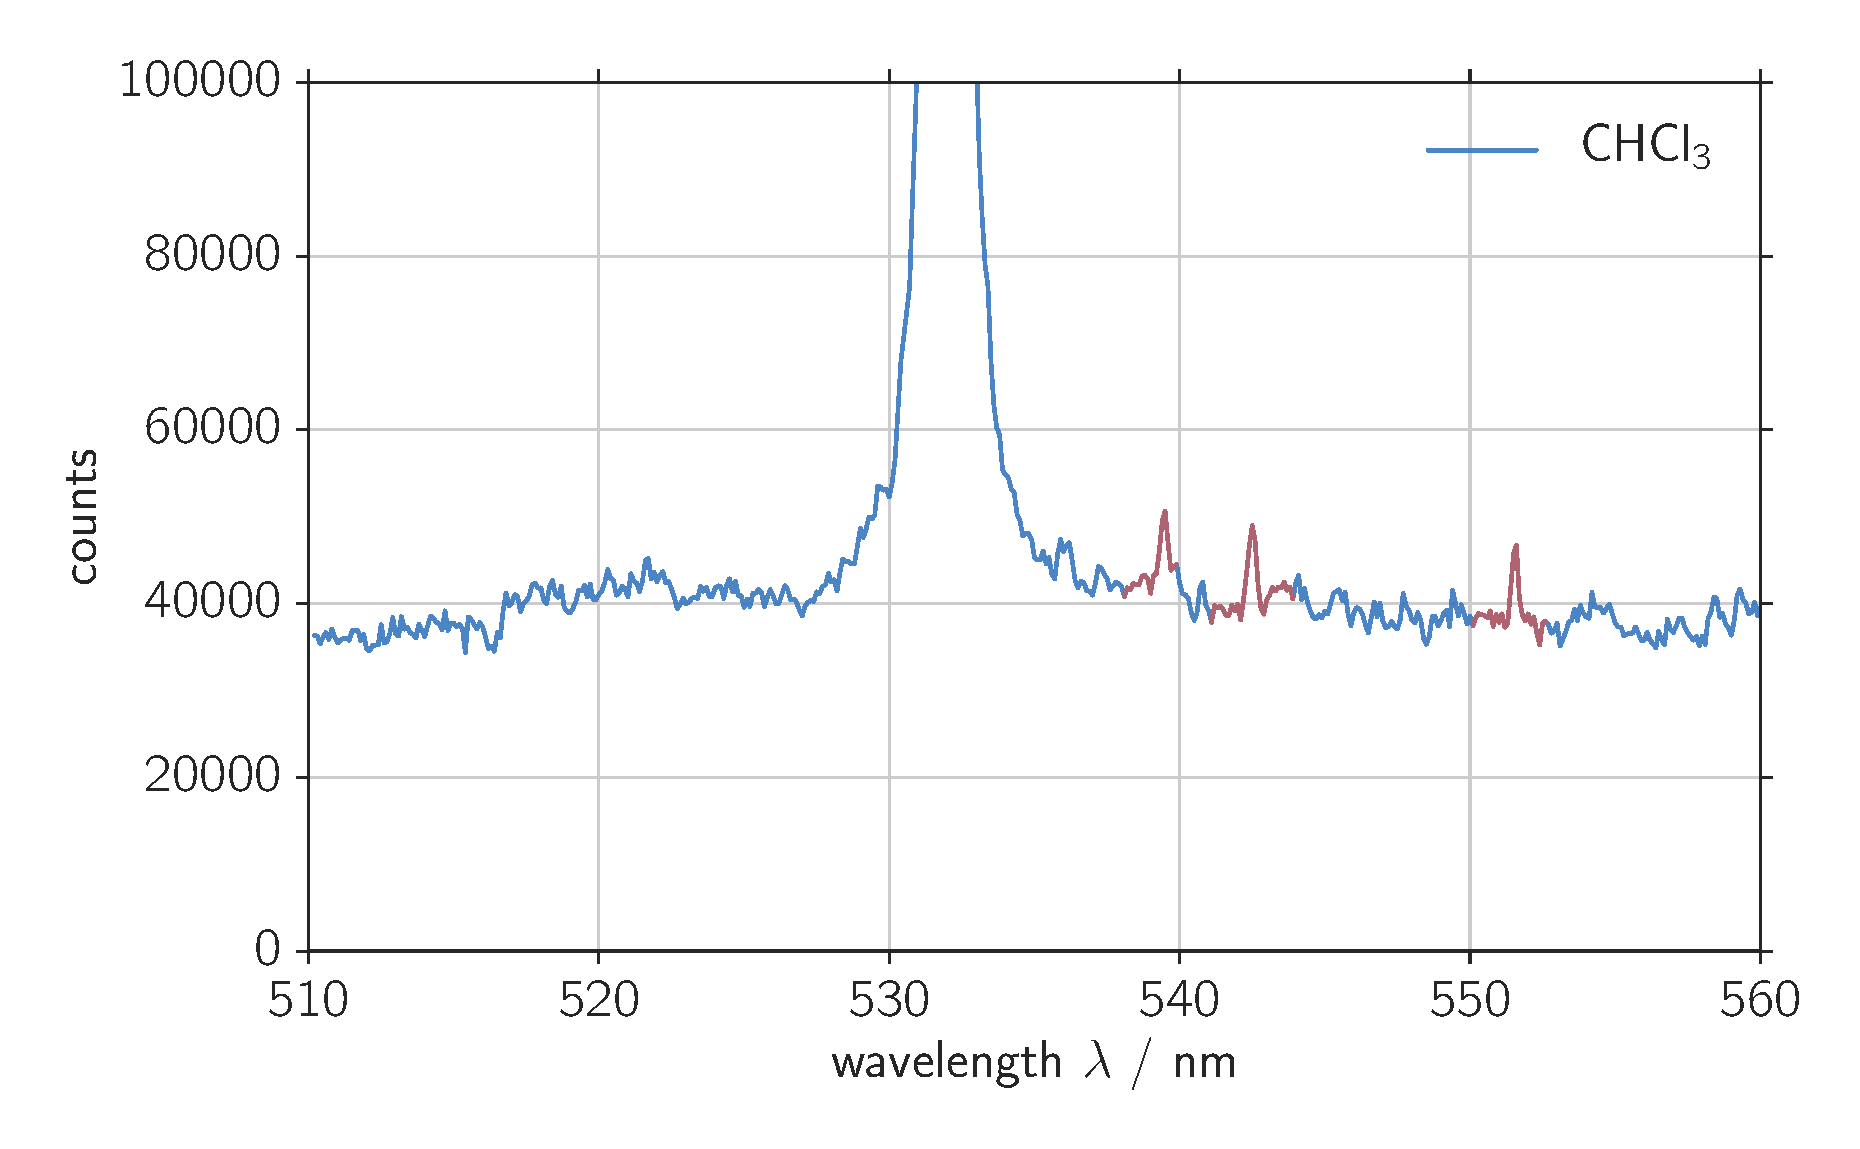
\includegraphics[width=0.8\linewidth]{analysis/figures/mono_chcl3}
    \caption{Spectrum of chloroform -- overview. The Rayleigh peak is cut off in order to make visible the less obvious 
    features. Three Stokes peaks are visible (highlighted), even though the signal-to-noise ratio is not satisfying.}
    \label{fig:mono_chcl3}
\end{figure}

\begin{table}[htpb]
    \centering
    \caption{
        Stokes peaks for chloroform (CHCl$_3$). 
        }
    \label{tab:mono_chcl3}
    \begin{tabular}{l r r r}
        \rowcolor{LightCyan} Peak N$^o$ & $\lambda \, / \, \text{nm}$ &
        $\Delta \nu \, / \, \text{ cm}^{-1}$ & 
        $\Delta \nu_\text{lit} \, / \, \text{ cm}^{-1}$ \\
        \cellcolor{LightCyan}$1$ & $539.5 \pm 0.2$ & $257 \pm 11$ & $260$   \\
        \cellcolor{LightCyan}$2$ & $542.5 \pm 0.2$ & $360 \pm 11$ & $366$   \\
        \cellcolor{LightCyan}$3$ & $551.6 \pm 0.2$ & $664 \pm 11$ & $680$  
    \end{tabular}
\end{table}

The third spectrum measured with the monochromator is that of carbon tetrachloride (CCl$_4$) and is shown in figure 
\ref{fig:mono_ccl4}. Here we display a measurement done with a much lower voltage applied to the photomultiplier, 
namely 679~V. The sampling speed was again 0.1~\AA/s. One can immediately notice the much lower count rates, both for 
the background and the signals. However, the signal-to-noise ratio does not change considerably. By eye, we identify 
three Stokes and on Anti-Stokes peak. The result of the quantitative analysis is shown in table \ref{tab:mono_ccl4}. 
All four peaks cover the literature values within their error.

\begin{figure}[htpb]
    \centering
    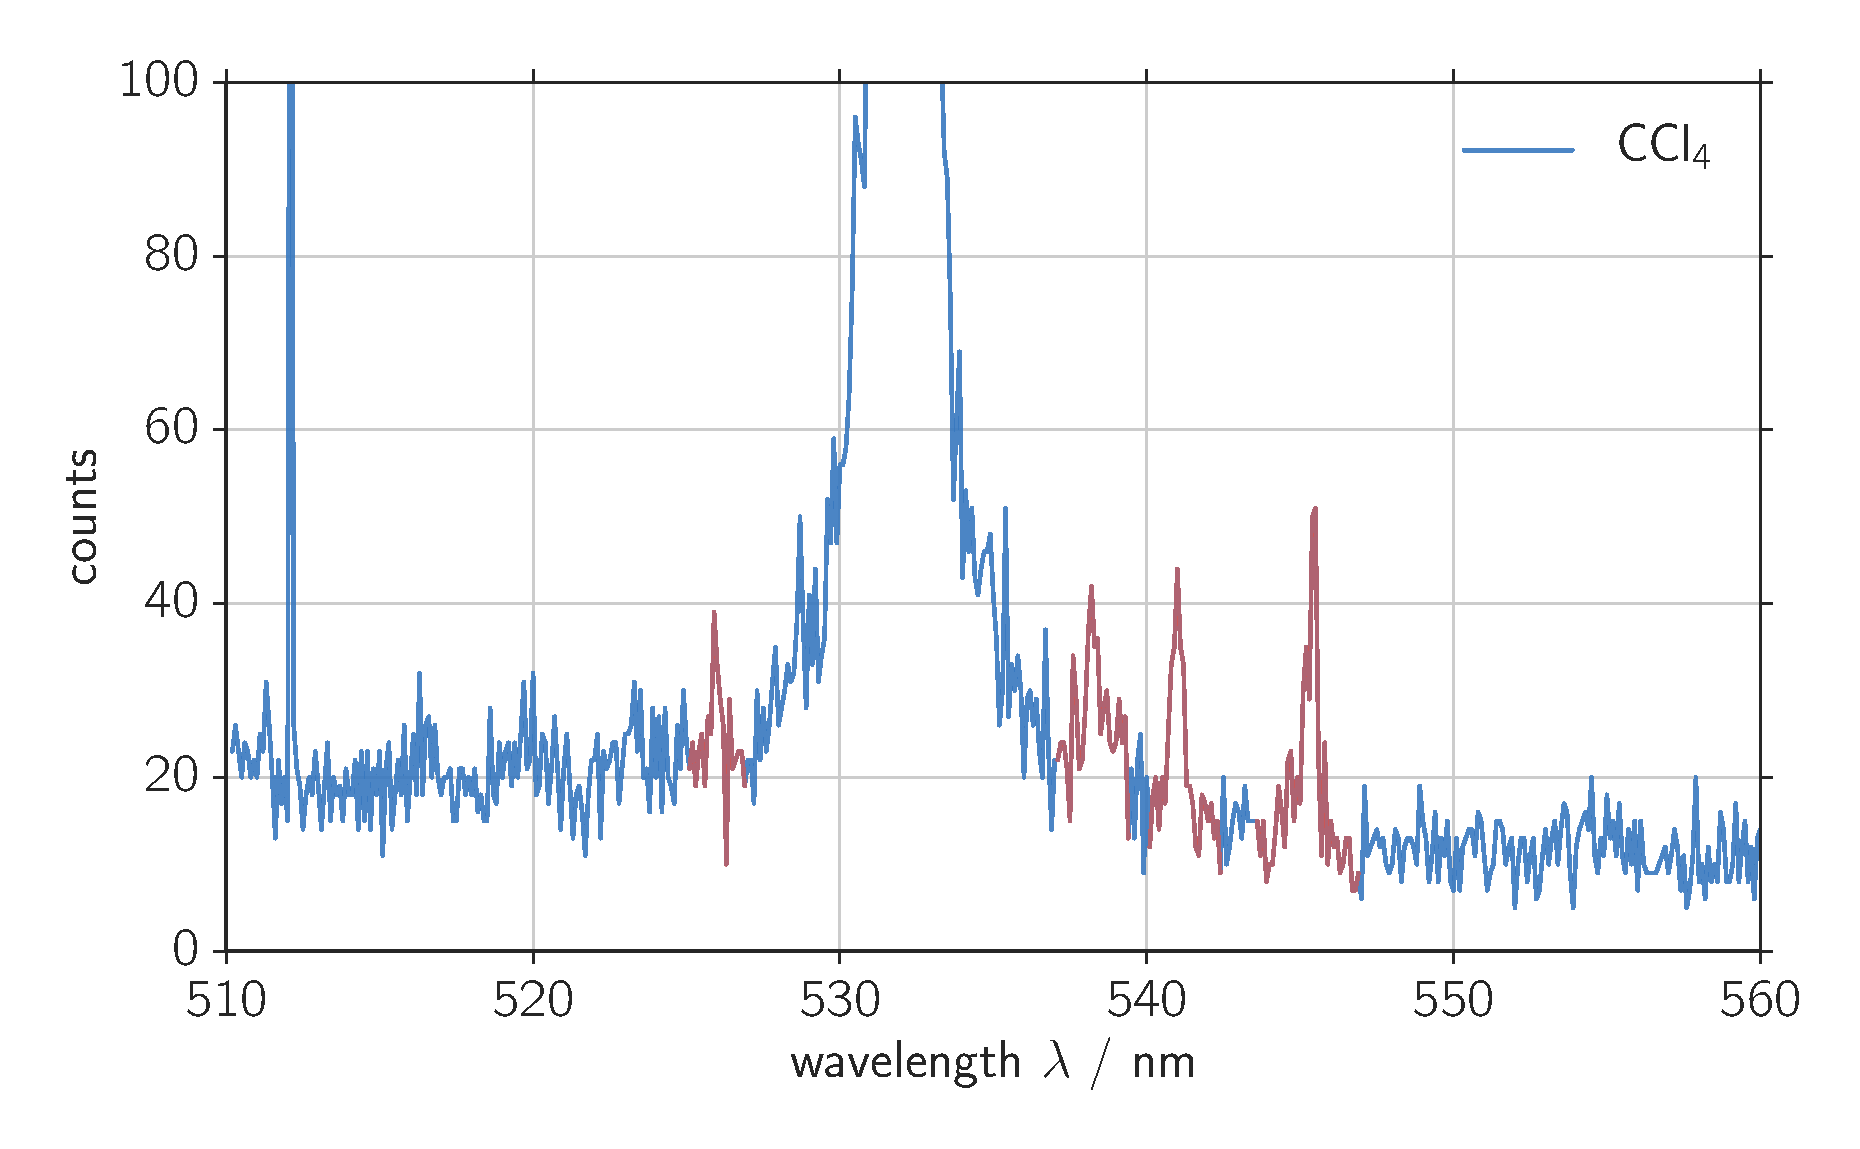
\includegraphics[width=0.8\linewidth]{analysis/figures/mono_ccl4}
    \caption{Overview over spectrum of CCl$_4$ taken with the monochromator. Note the much lower count numbers due to 
    the reduces voltage at the photomultiplier (679 V instead of the previously used 1000 V). Signal-to-noise ratio is 
    not considerably reduced. However, four Raman peaks are visible (highlighted). }
    \label{fig:mono_ccl4}
\end{figure}

\begin{table}[htpb]
    \centering
    \caption{
        Identified Raman peaks for carbon tetrachloride (CCl$_4$). 
        }
    \label{tab:mono_ccl4}
    \begin{tabular}{l r r r}
        \rowcolor{LightCyan} Peak N$^o$ & $\lambda \, / \, \text{nm}$ &
        $\Delta \nu \, / \, \text{ cm}^{-1}$ & 
        $\Delta \nu_\text{lit} \, / \, \text{ cm}^{-1}$ \\
        \cellcolor{LightCyan}Anti-Stokes& && \\
        \cellcolor{LightCyan}$1$ & $525.9 \pm 0.2$ & $222 \pm 12$ & $217$   \\
        \cellcolor{LightCyan}Stokes& && \\
        \cellcolor{LightCyan}$2$ & $538.2 \pm 0.2$ & $212 \pm 12$ & $217$   \\
        \cellcolor{LightCyan}$3$ & $541.0 \pm 0.2$ & $309 \pm 11$ & $314$   \\
        \cellcolor{LightCyan}$4$ & $545.5 \pm 0.2$ & $461 \pm 11$ & $459$ 
    \end{tabular}
\end{table}



\subsection{CCD spectrometer}
The CCD spectrometer yielded much better results in terms of signal-to-noise ratio and usable intensity measurements. 
Most notable, the resolution in wavelength is much higher, such that the finite width of the peaks can be resolved.
This allows fitting for all peaks. We fitted on a scaled Breit-Wigner distribution plus an offset, 
\begin{equation}
    r(\lambda) = \frac{A}{\pi \gamma \left[1 + \left(\frac{\lambda - \lambda_0}{\gamma}\right)^2\right]} + B, 
\end{equation} 
where r is the measured rate, A the scale factor, $\gamma$ and $\lambda_0$ the parameters of the Breit-Wigner 
distribution and B the offset rate. The integral over the Breit-Wigner distribution equals one, such that we can use the 
scale factor as the intensity of the peak. 
We ignored the small error induced by the fact the we applied the function on the distribution over wavelength, although 
the theoretical results are only valid for the distributions over frequencies. Errors on wavelength are ignored 
for the fit, while those on count rates are derived from the statistical errors on the original counts $N$, namely 
\begin{equation}
    s_r = \sqrt{N} / t
\end{equation}
with integration time t. For those measurements where we subtract the background or correct for detection probability, 
the errors are adapted according to Gaussian error propagation. 

The only mayor problem when using the CCD is the effect of overflow: Once the cells corresponding to one wavelength 
are saturated, they induce a current to neighboring cells. Thus, a peak with high intensity will be measured much 
broader. Since the Raman peaks are much less intensive then the Rayleigh peak, those close to the latter will be 
'swallowed' by the overflow. To avoid this, we use a notch filter, which suppresses the radiation in a fixed range.
This range, however, also includes some of the Raman peaks too close to the Rayleigh peak. 

\subsubsection{Calibration}
The course of the calibration goes analogously with the previous one. The result can be seen in figure 
\ref{fig:ccd_calibration_hg}. The measurement time was 5 $\mu$s, we averaged 1000 measurements. 
The fit results and their literature counterparts are shown in table \ref{tab:mono_calibration}.  
For a more thorough analysis, we apply a linear regression on the measured peaks. The result is shown in 
figure \ref{fig:ccd_calibration_fit}. Quite visibly, the calibration of the CCD spectrometer is correct. 
In the following sections, we will apply the linear function to the wavelength at the center of each peak before. 
This will also result in an error on the wavelength: In the range in question (400 to 600 nm), this error is 
0.3 to 0.5 nm. 

\begin{table}[htpb]
    \centering
    \caption{
        Peaks of Hg-spectrum measured with the CCD. Notice the good agreement. This is further quantified in i
        a linear regression. 
        }
    \label{tab:mono_calibration}
    \begin{tabular}{c r r}
        \rowcolor{LightCyan} Peak & $\lambda_\text{a} \,/\, \text{nm}$ & $\lambda_\text{lit} \,/\, \text{nm}$ \\
        \cellcolor{LightCyan}$1$ & $435.5 \pm 0.3$ & $435.8$   \\
        \cellcolor{LightCyan}$2$ & $545.9 \pm 0.3$ & $546.1$   \\
        \cellcolor{LightCyan}$3$ & $576.8 \pm 0.3$ & $577.1$   \\
        \cellcolor{LightCyan}$4$ & $578.9 \pm 0.3$ & $579.1$   
    \end{tabular}
\end{table}

\begin{figure}[htpb]
    \centering
    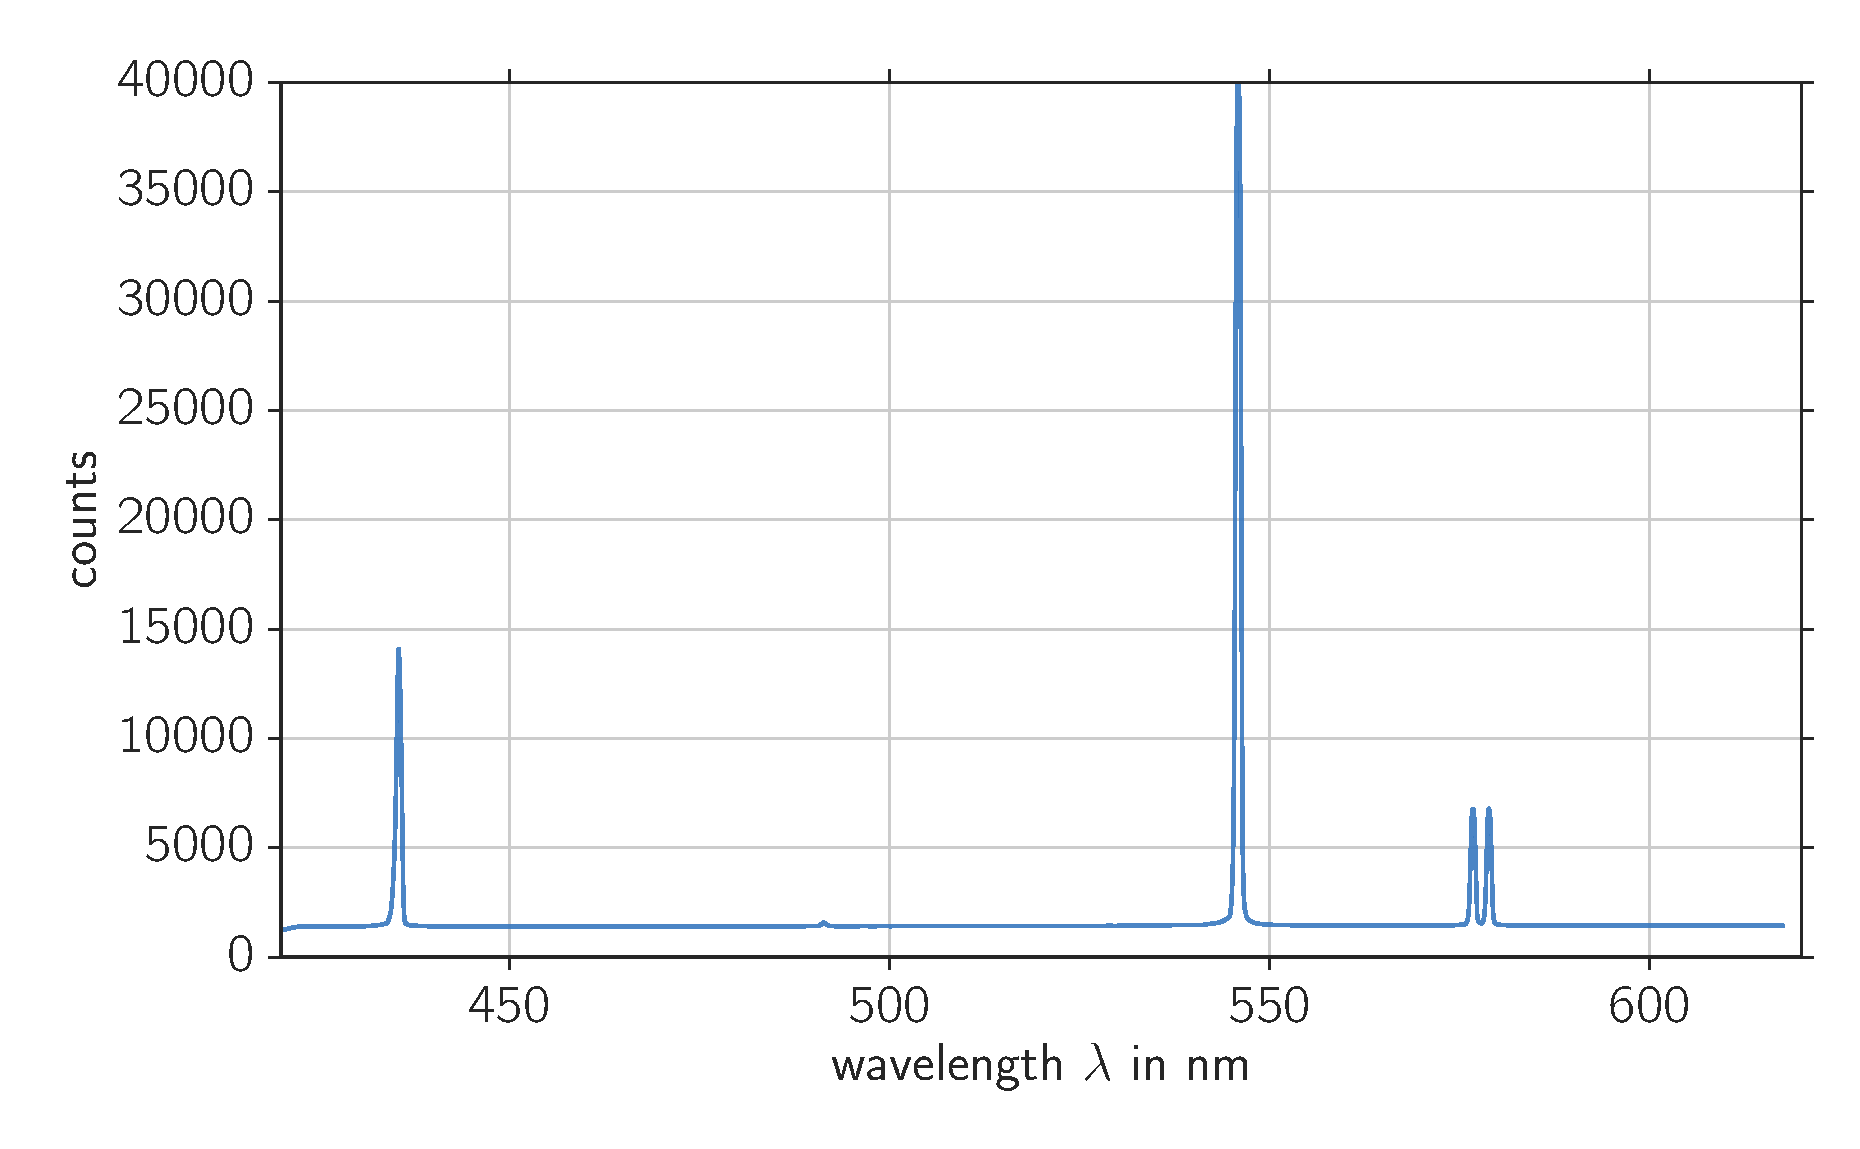
\includegraphics[width=0.8\linewidth]{analysis/figures/ccd_calibration_hg}
    \caption{Hg spectrum recorded with CCD. Peaks are fitted with a Breit-Wigner distribution.}
    \label{fig:ccd_calibration_hg}
\end{figure}

\begin{figure}[htpb]
    \centering
    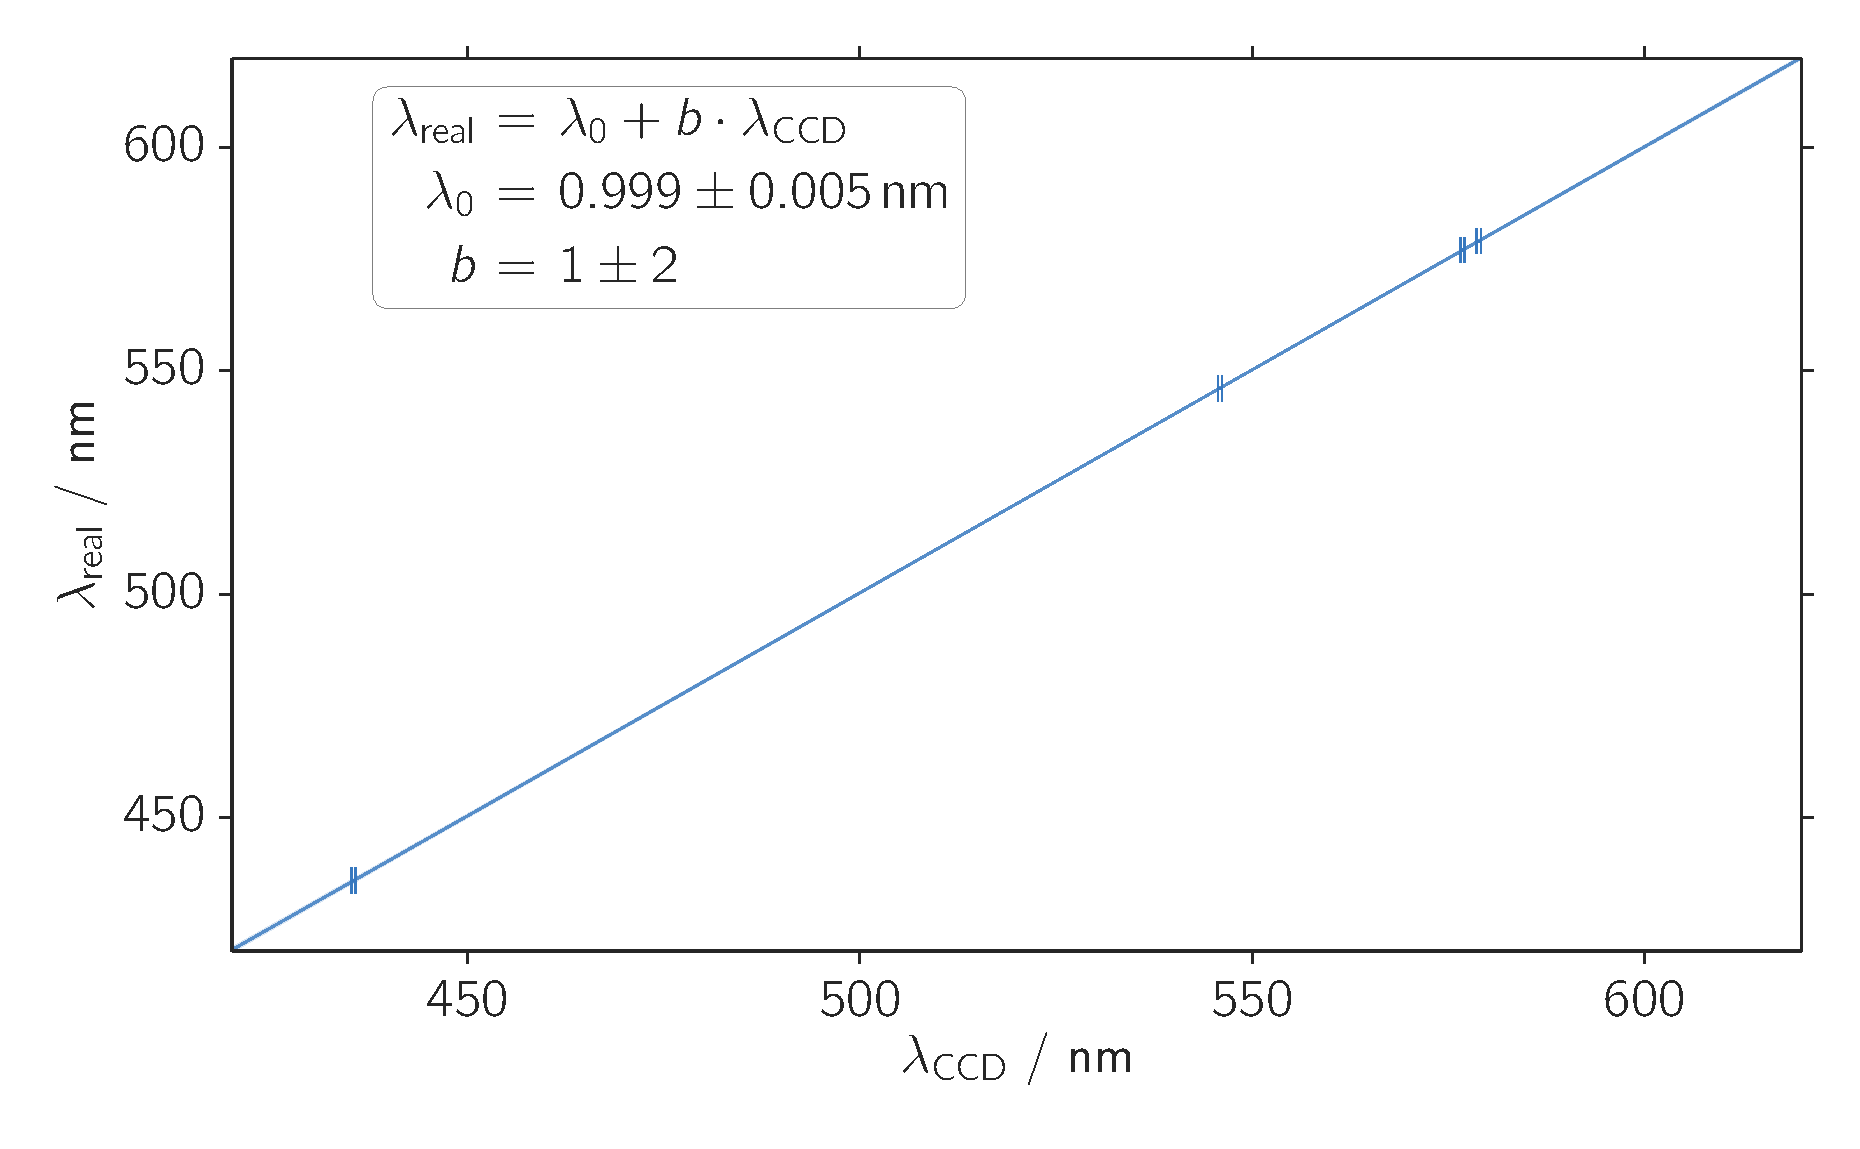
\includegraphics[width=0.8\linewidth]{analysis/figures/ccd_calibration_fit}
    \caption{Linear fit on fitted Hg peaks over literature values. The correspondence is nearly one-to-one. }
    \label{fig:ccd_calibration_fit}
\end{figure}


\subsubsection{Detection probability of polarized light}
In order to examine the detection probability for polarized light for the CCD, we compare measurements with 
a polarization filter in front of the spectrometer in three different positions: $0^\circ, 45^\circ$ and 
$90^\circ$. The measurements are plotted in figure \ref{fig:ccd_polarized} and show similar but more regular 
behavior like the monochromator. The spikes are defects appearing at the same positions in various following 
measurements. In figure \ref{fig:ccd_correction} we display a correction factor derived from those 
measurements. We take the measurement at $45^\circ$ as a reference value and rescale the measurements with
vertical and horizontal polarization to this value at each wavelength $\lambda$. In order to minimize the 
effects of noise, we applied a Savitzky-Golay filter with a width of 301 points and a fourth degree polynomial
to the data (see \cite{scipy} for reference). This filtered correction factor is applied on the data in the 
upcoming analysis. 

\begin{figure}[htpb]
    \centering
    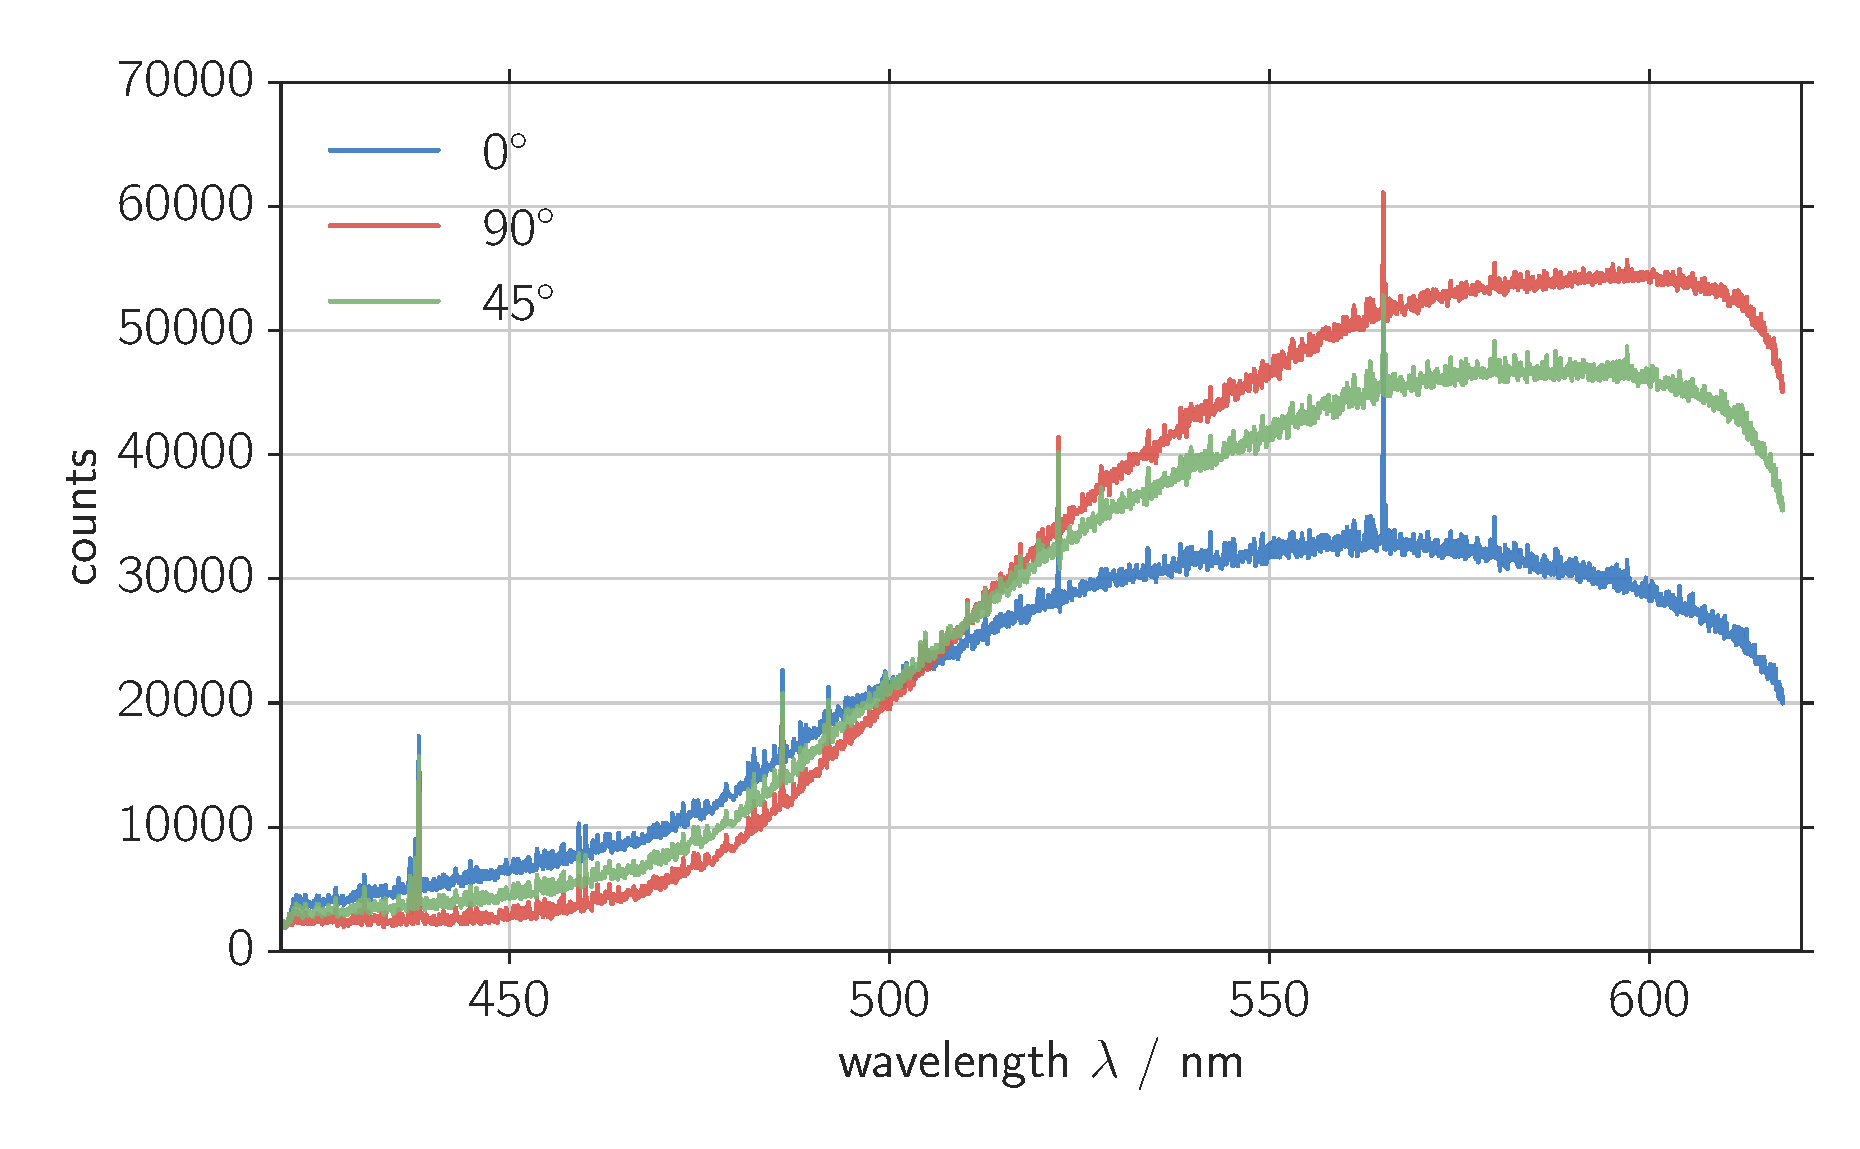
\includegraphics[width=0.8\linewidth]{analysis/figures/ccd_polarized}
    \caption{Spectrum of white light polarized at different angles measured with the CCD. The $45^\circ$ value
    is taken as a reference to derive the correction factor. Single spikes are defects and taken out in the 
    future analysis.}
    \label{fig:ccd_polarized}
\end{figure}

\begin{figure}[htpb]
    \centering
    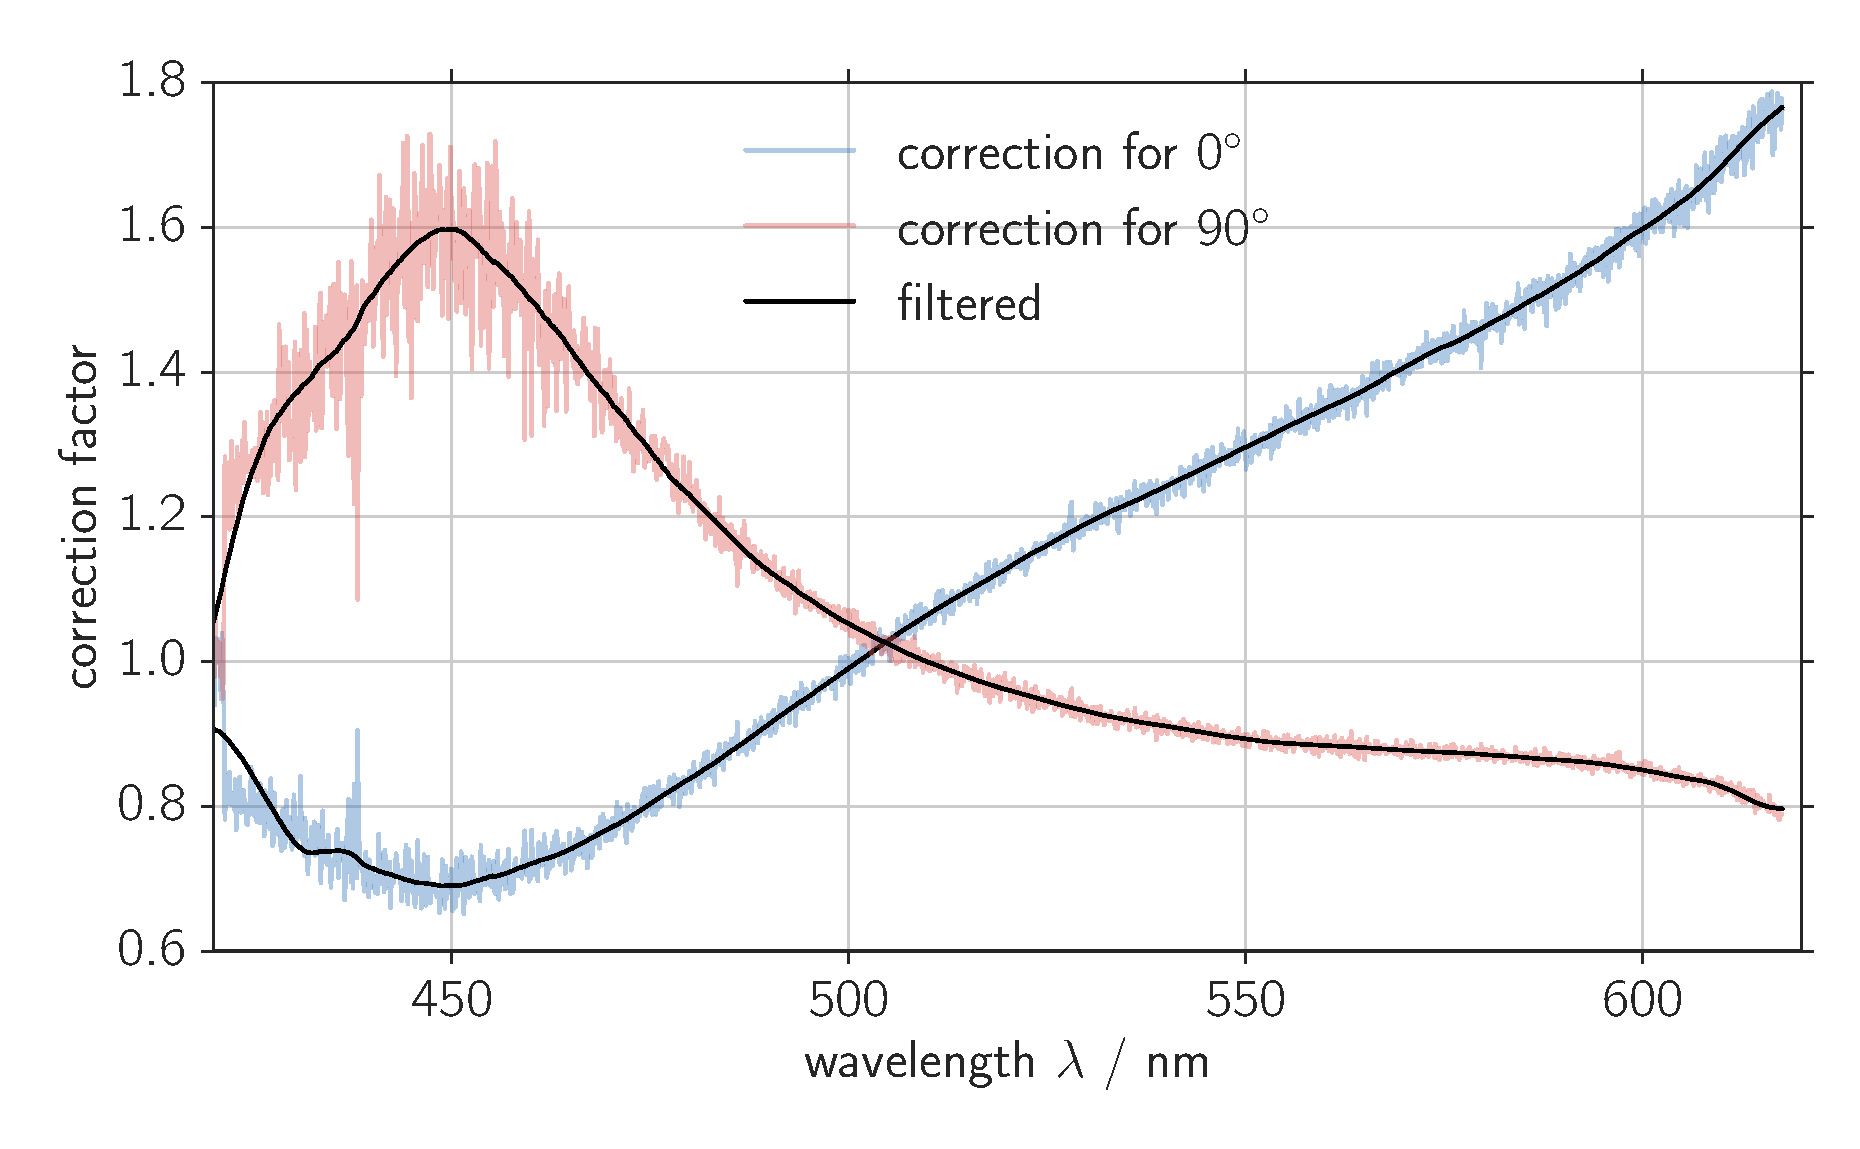
\includegraphics[width=0.8\linewidth]{analysis/figures/ccd_correction}
    \caption{CCD correction factors for polarization bias. The factor is calculated as 
        $\frac{r_{45^\circ}(\lambda)}{r_\text{measured}(\lambda)}$. The raw data is filtered in order to minimized 
    the effects of noise.}
    \label{fig:ccd_correction}
\end{figure}

\subsubsection{Analysis of laser}
\label{sec:laser}
The laser was not analyzed directly since its intensity is too high for the sensitive devices used. Instead we 
analyzed the Rayleigh peak with carbon tetrachloride as a sample. The measurement for 5 $\mu$s was averaged 1000
times, results can be observed in figure \ref{fig:ccd_laser_peak}. The data is fitted on a scaled gaussian with 
offset yielding a central value of $\lambda_0 = 532.1 \pm 0.3$. This is in good agreement with the declaration 
of the manufacturer, stating a wavelength of 532 nm. 


\begin{figure}[htpb]
    \centering
    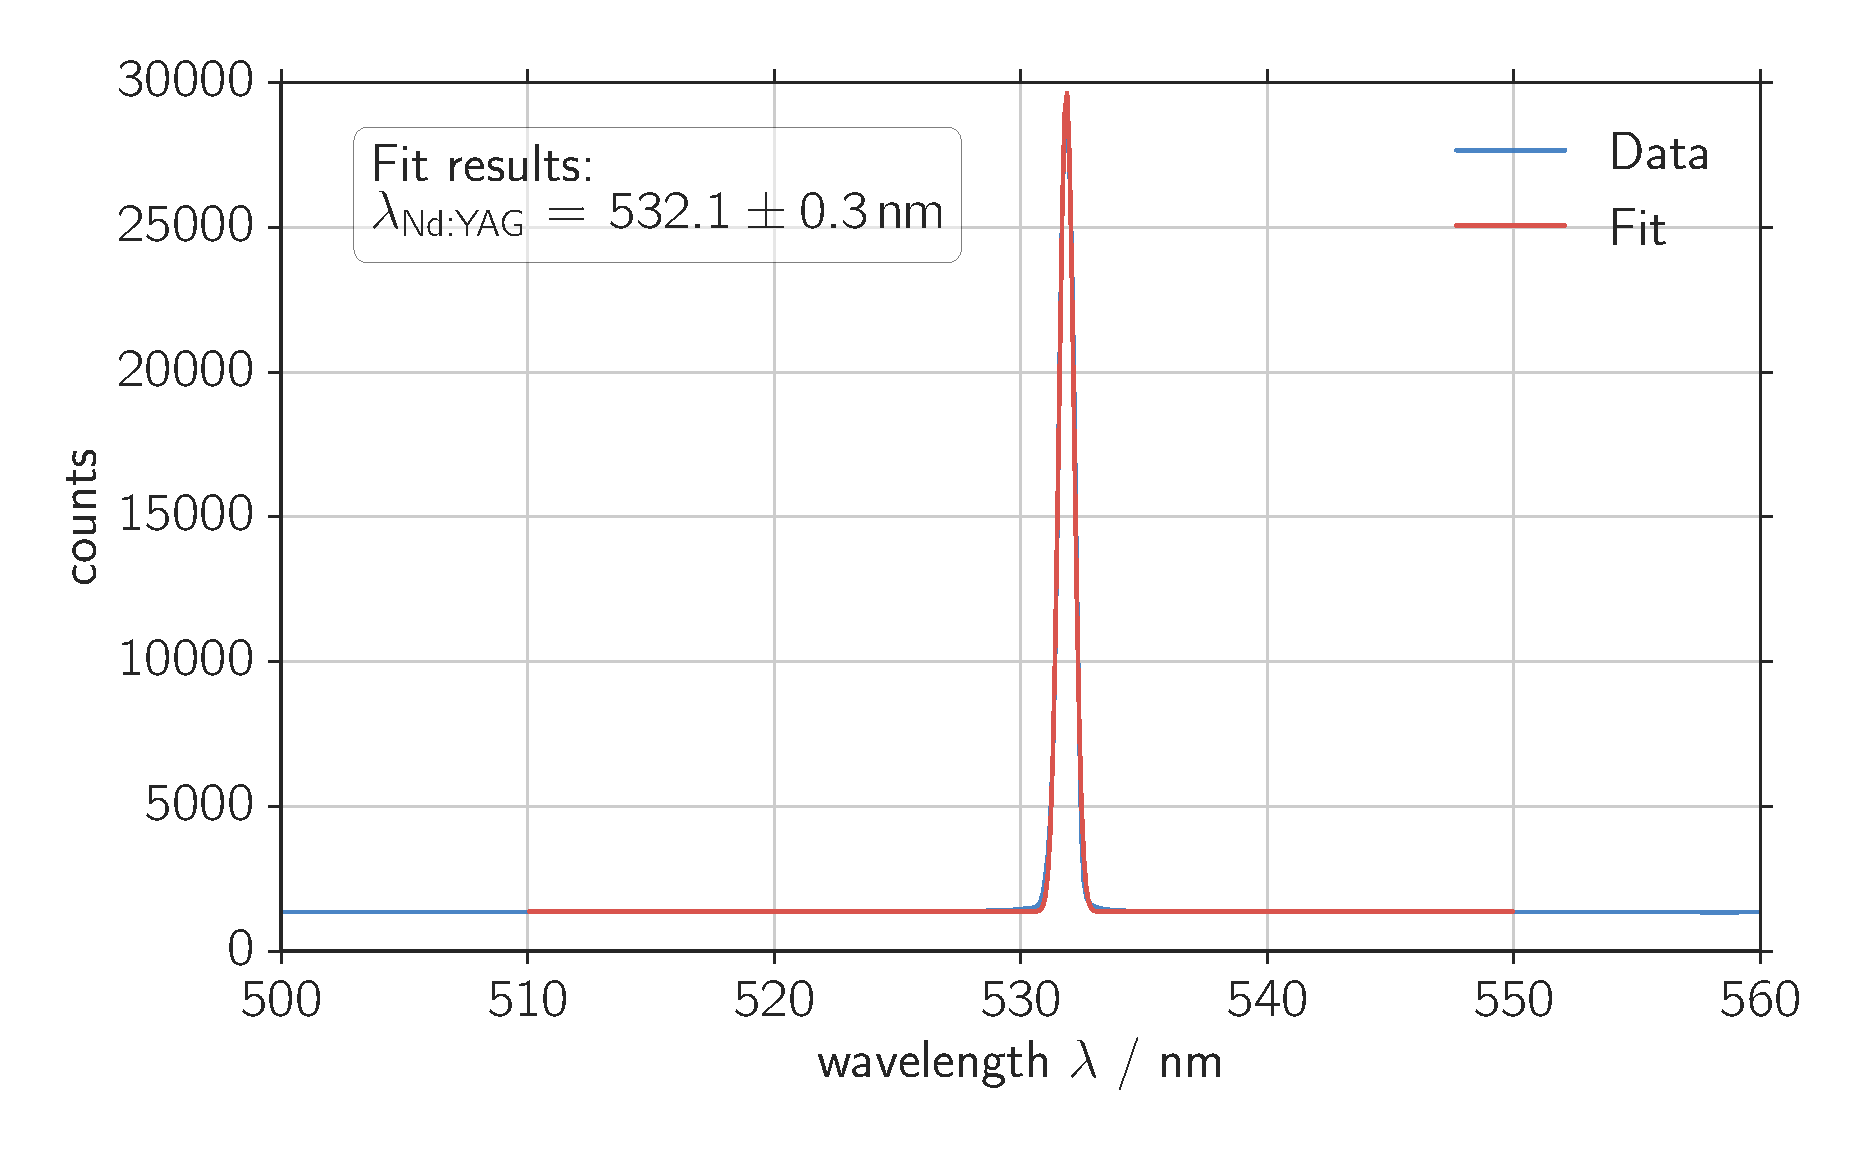
\includegraphics[width=0.8\linewidth]{analysis/figures/ccd_laser_peak}
    \caption{Measurement of laser peak. The data corresponds to the Rayleigh peak of the frequency doubled Nd:YAG 
    laser with CCl$_4$ as the scattering sample. The fit is a gaussian, yielding a central wavelength of 
$\lambda_0 = (532.1 \pm 0.3)$ nm in good accordance with the given value. }
    \label{fig:ccd_laser_peak}
\end{figure}

\subsubsection{Notch filter}
In this section we investigate the effect of the notch filter on the spectrum. We use white light as a source and 
plot the resulting spectrum in figure \ref{fig:ccd_notch_filter}. For direct comparison, we also plot a rescaled 
measurement of the unfiltered white light. One can observe the sharp restriction of the filter for wavelength 
between 524 and 541 nm. A closer look on the edges (not shown) reveals some substructure. However, these features 
will be neglected in the ongoing analysis. Instead, we will repeatedly include the difference between rescaled 
unfiltered and filtered spectrum in the following plots in order to distinguish real peaks from artifacts induced 
by the filter. 

\begin{figure}[htpb]
    \centering
    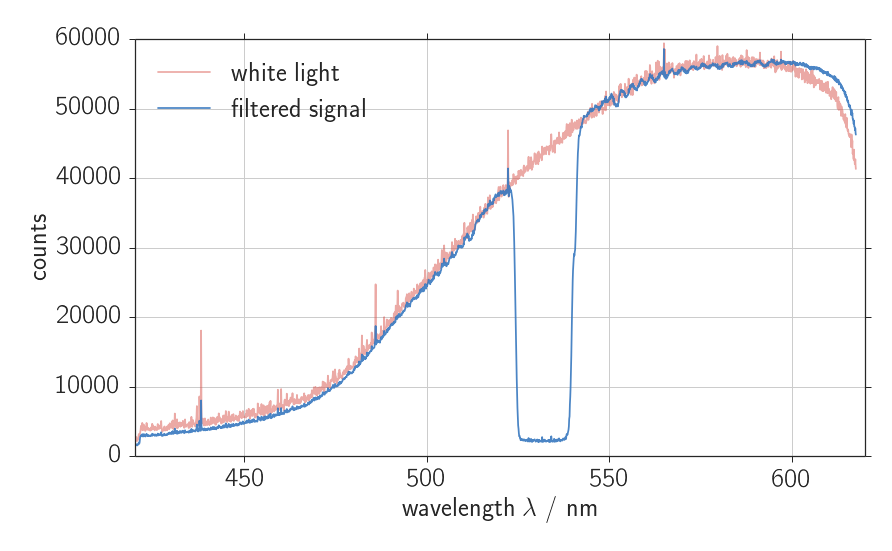
\includegraphics[width=0.8\linewidth]{analysis/figures/ccd_notch_filter}
    \caption{Effect of the notch filter on the spectrum of white light. The unfiltered spectrum is rescaled for 
    better comparability. Effects at the edges of the filter are neglected as we exclude features in this region
    from further analysis in any case.}
    \label{fig:ccd_notch_filter}
\end{figure}

\subsection{Main analysis}
In this section we apply the obtained results of the previous one in order to investigate various spectra of 
Raman-active samples. As a first step, the background rate is measured with the laser turned on but without
a sample inserted. We set a measurement time of 30 s and averaged 10 measurements. The counts are transferred 
to rates and subtracted from all following measurements. 

\subsubsection{Spectra of CS$_2$ and CHCl$_3$}
For both samples, the spectra are recorded with a laser current of 1.50 A and with the notch filter installed. 
Integration times were set to 10 s (CS$_2$ with $\lambda / 2$ plate: 5 s), we did not average. We fit peaks in
manually defined ranges. For carbon disulfide, peaks were visible for both the measurement without $\lambda / 2$ 
plate and the one with the plate (see figure \ref{fig:ccd_cs2_spectra}). The fit results are averaged and presented 
in table \ref{tab:ccd_cs2_peaks}. The first Stokes and the Anti-Stokes peaks are in good agreement with the 
literature value. The second Stokes peak is not close to any literature values we found. Our source lists three
vibrational modes at 658, 1535 and $397 \text{cm}^{-1}$. The reason for this disagreement could be another 
substance within the sample inducing this Raman peak. There could further be other experimental problems, or
(unlikely) missing data in our source. 

The chloroform measurement without $\lambda / 2$ plate yielded a number of visible peaks: One can observe 
four Stokes peaks and three Anti-Stokes peaks, refer to figure \ref{fig:ccd_chcl3_spectra}. This is expected
as the molecule has more degrees of freedom than the linear CS$_2$ molecule. Fit results and literature 
values are shown in table \ref{tab:ccd_chcl3_peaks}. The peaks at 366 and $1220 \text{ cm}^{-1} $ are
found within the standard deviation, the peaks at 680 and 774 are either met or measured with a lower wavenumber
(just above one sigma). In general, we observe a tendency for the wavenumbers to be too low. This would imply
peaks closer to the Rayleigh peak then the values measured in literature. And explanation for this phenomenon 
would require a closer investigation of the used equipment. 
\begin{table}[htpb]
    \centering
    \caption{
        Measured Raman peaks with CS$_2$ sample. The values two measurements are averaged. 
        Note that one peak does not have a literature counterpart. This peak might be due to another 
        substance. 
        }
    \label{tab:ccd_cs2_peaks}
    \begin{tabular}{l r r r}
        \rowcolor{LightCyan} Peak N$^o$ & $\lambda \, / \, \text{nm}$ &
        $\Delta \nu \, / \, \text{ cm}^{-1}$ & 
        $\Delta \nu_\text{lit} \, / \, \text{ cm}^{-1}$ \\
        \cellcolor{LightCyan}Anti-Stokes &&& \\
        \cellcolor{LightCyan}$1$ & $514.256 \pm 0.003$ & $652 \pm 11$ & $658$   \\
        \cellcolor{LightCyan}Stokes &&& \\
        \cellcolor{LightCyan}$2$ & $551.232 \pm 0.002$ & $652 \pm 11$ & $658$   \\
        \cellcolor{LightCyan}$3$ & $555.716 \pm 0.003$ & $799 \pm 11$ & $?$  
    \end{tabular}
\end{table}

\begin{figure}[htpb]
    \centering
    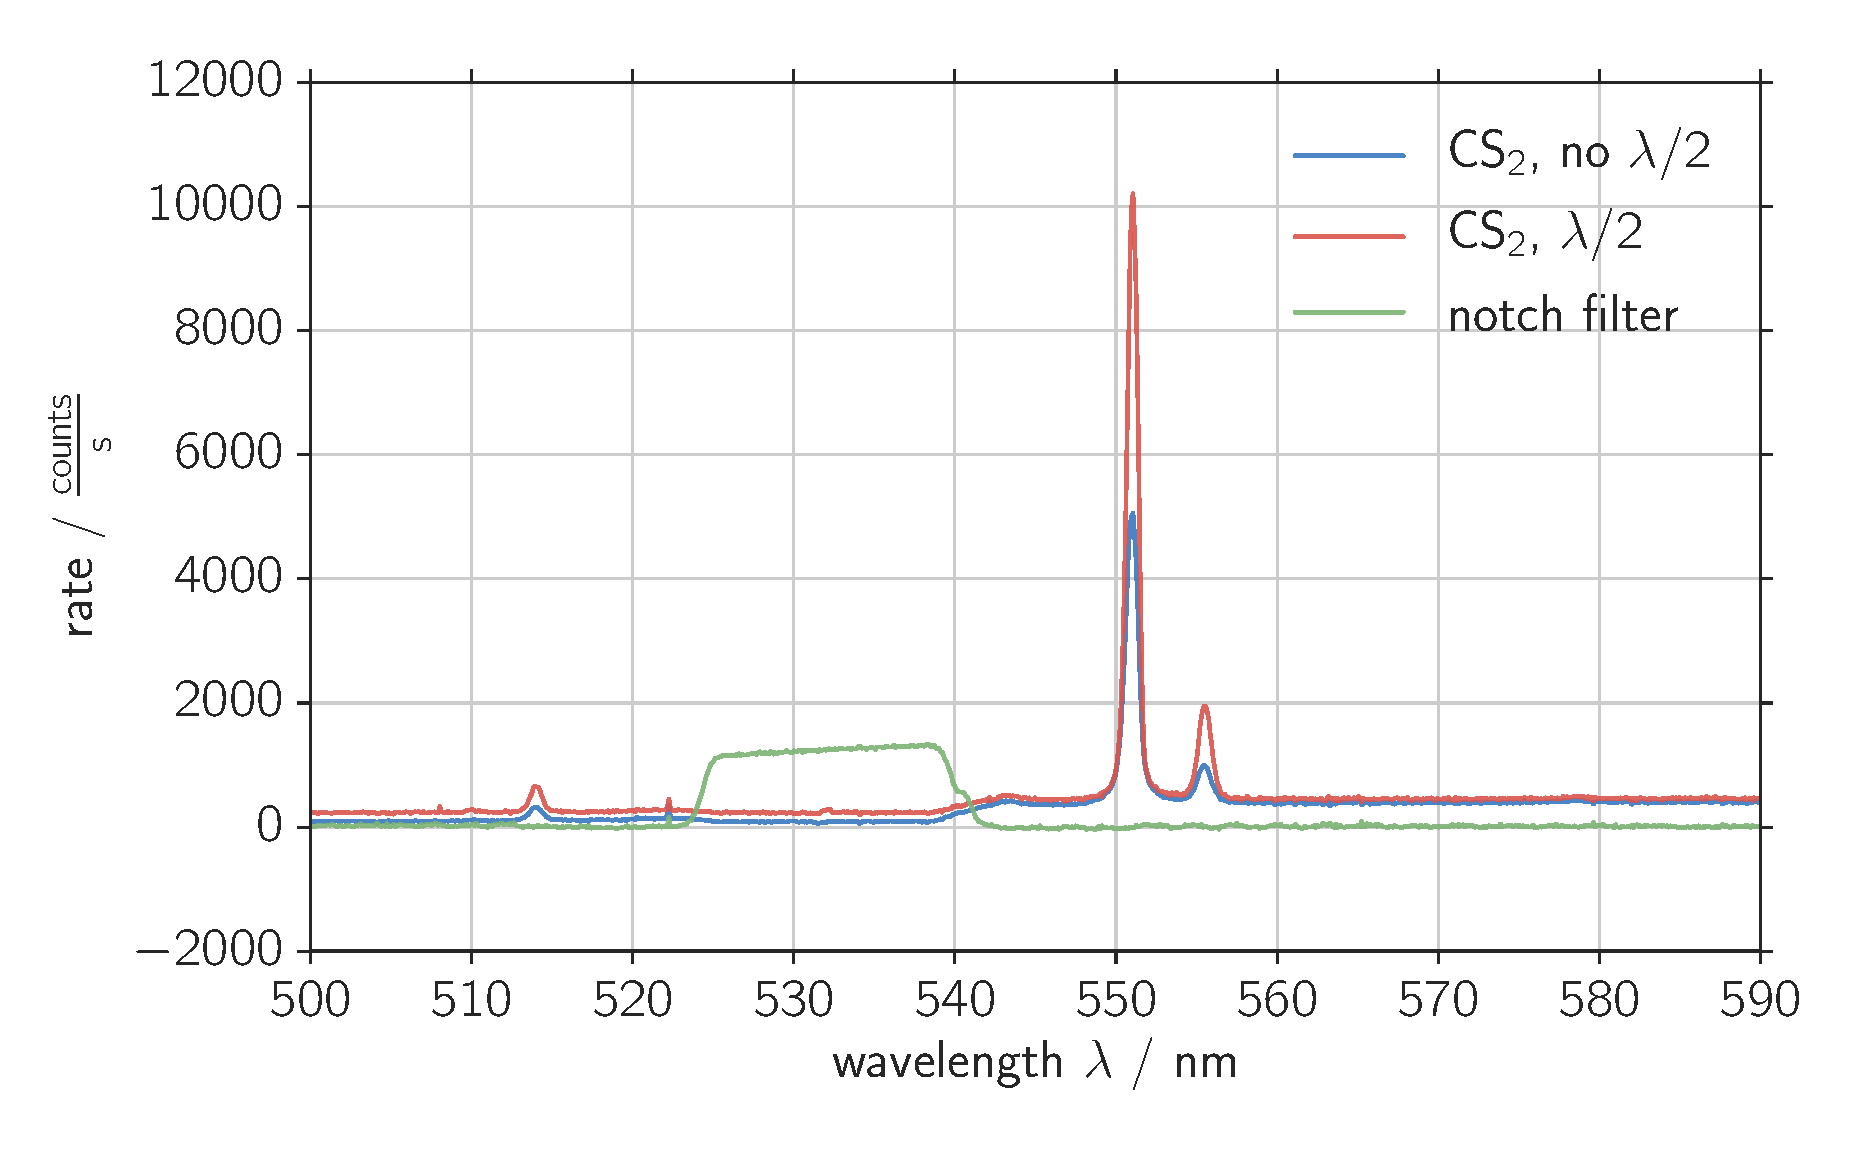
\includegraphics[width=0.8\linewidth]{analysis/figures/ccd_cs2_spectra}
    \caption{
        Spectrum of carbon disulfide, recorded with the CCD spectrometer. 
        The higher intensities are recorded witht he $\lambda / 2$ plate installed, 
        due to the vertical polarization of the laser. The effect of the notch filter
        is plotted for an easier interpretation of the data.}
    \label{fig:ccd_cs2_spectra}
\end{figure}

\begin{table}[htpb]
    \centering
    \caption{
        Raman peaks measured with the chloroform sample. Literature values are not always met. In general the 
        measured values for the wavenumbers are too small.
        }
    \label{tab:ccd_chcl3_peaks}
    \begin{tabular}{l r r r}
        \rowcolor{LightCyan} Peak N$^o$ & $\lambda \, / \, \text{nm}$ &
        $\Delta \nu \, / \, \text{ cm}^{-1}$ & 
        $\Delta \nu_\text{lit} \, / \, \text{ cm}^{-1}$ \\
        \cellcolor{LightCyan}Anti-Stokes &&& \\
        \cellcolor{LightCyan}$1$ & $511.4 \pm 0.8$ & $760 \pm 30$ & $774$   \\
        \cellcolor{LightCyan}$2$ & $513.8 \pm 0.3$ & $670 \pm 20$ & $680$   \\
        \cellcolor{LightCyan}$3$ & $522.0 \pm 0.4$ & $370 \pm 20$ & $366$   \\
        \cellcolor{LightCyan}Stokes &&& \\
        \cellcolor{LightCyan}$4$ & $542.6 \pm 0.3$ & $365 \pm 15$ & $366$   \\
        \cellcolor{LightCyan}$5$ & $551.7 \pm 0.3$ & $667 \pm 15$ & $680$   \\
        \cellcolor{LightCyan}$6$ & $554.5 \pm 0.7$ & $760 \pm 20$ & $774$   \\
        \cellcolor{LightCyan}$7$ & $568.9 \pm 0.5$ & $1210 \pm 20$ & $1220$   
    \end{tabular}
\end{table}

\begin{figure}[htpb]
    \centering
    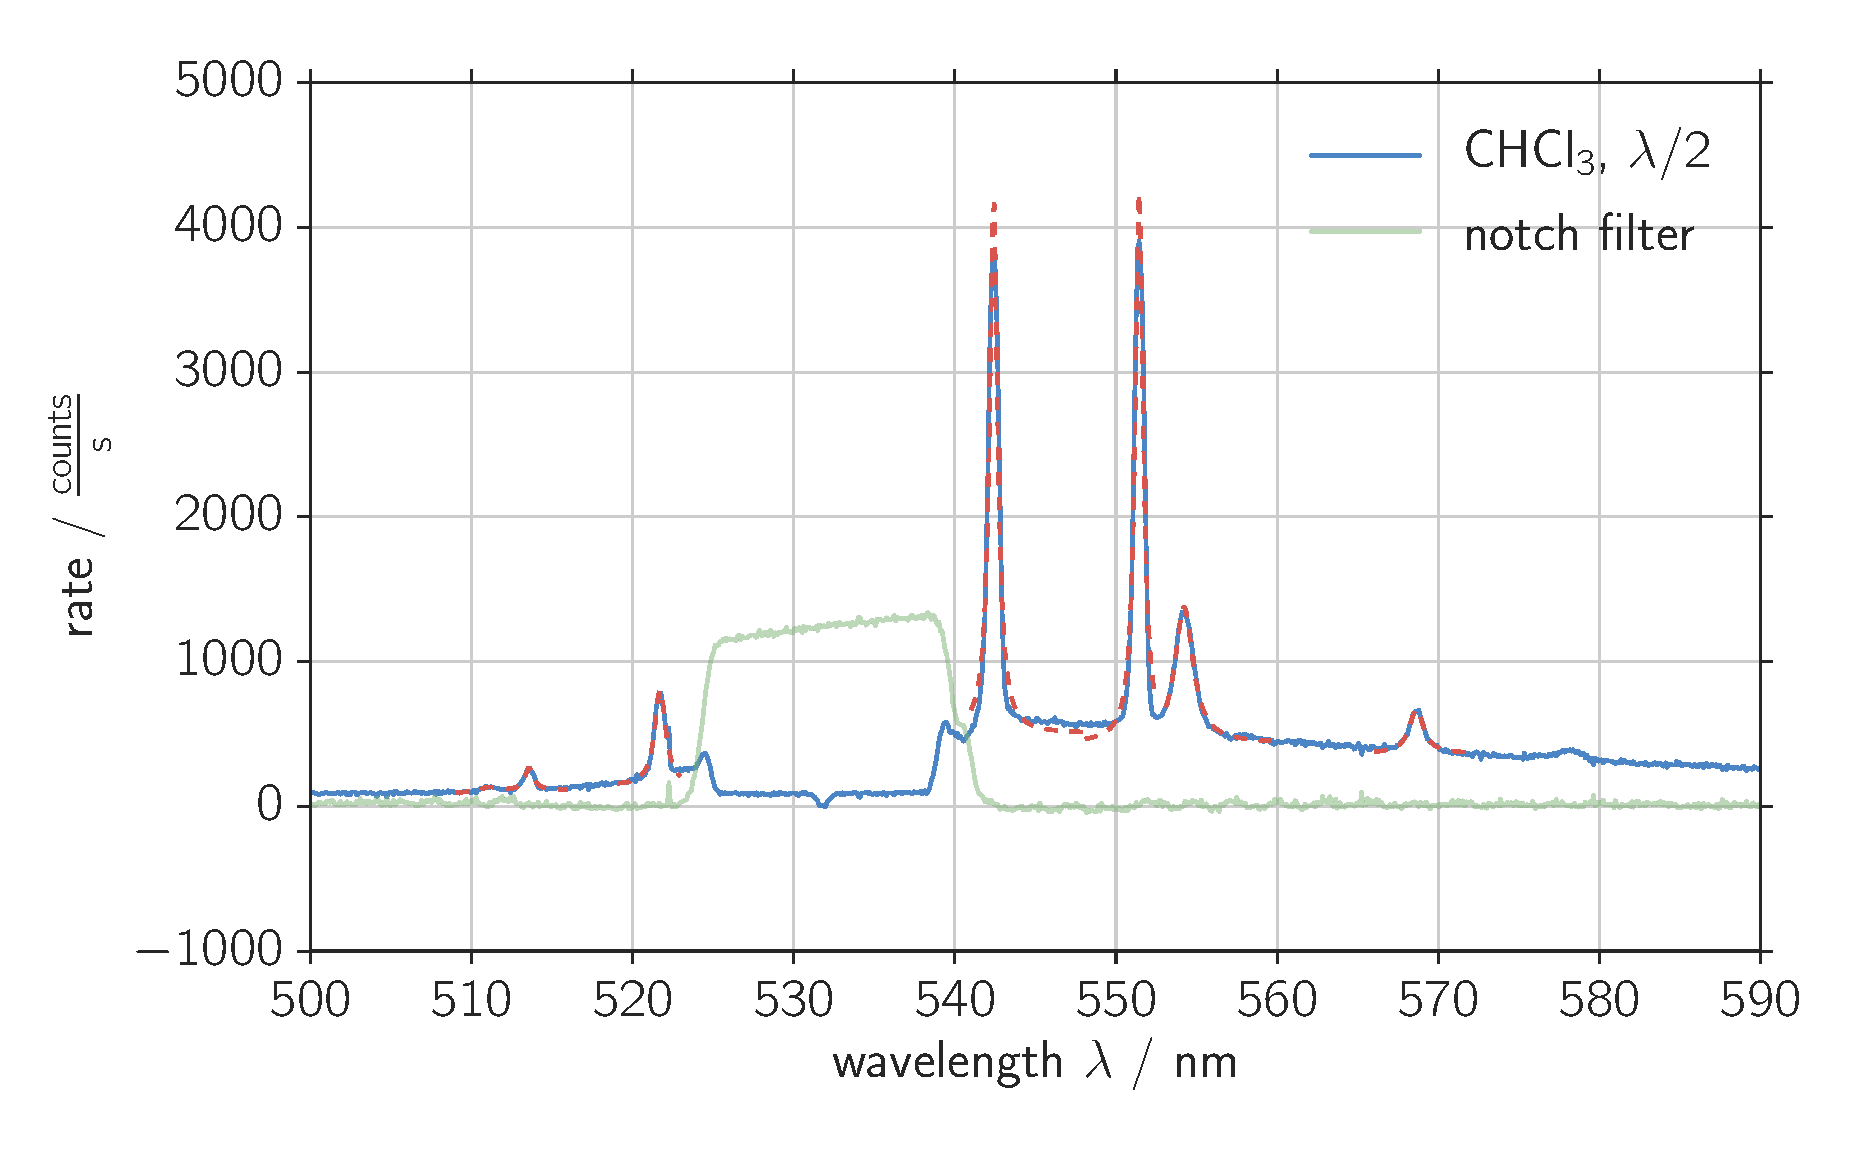
\includegraphics[width=0.8\linewidth]{analysis/figures/ccd_chcl3_spectra}
    \caption{
        Spectrum of chloroform measured with CCD and $\lambda / 2$ plate. We fitted four Stokes and 
        three Anti-Stokes peaks, fit results are plotted as dotted lines for illustration. The Anti-Stokes 
        peak at 511.4 nm is not visible on this scale. 
    }
    \label{fig:ccd_chcl3_spectra}
\end{figure}

\subsubsection{Spectrum of CCl$_4$ -- Depolarization}
The spectrum of carbon tetrachloride is analyzed more thoroughly in order to measure its depolarization. We used 
the notch filter and the $\lambda / 2$ plate. The laser current was left at 1.50 A. The polarization filter was 
used in two perpendicular positions, vertical and horizontal. Measurement time was set to 20 s, averaging over 
ten measurements. The resulting plot is shown in figure \ref{fig:ccd_ccl4_spectra} for both polarizations, fit results 
and peaks are listed in table \ref{tab:ccl4_peaks}. The first three Stokes and all Anti-Stokes peaks can be 
identified with the literature values within standard deviations. The fourth measured peak does not appear 
in the literature and may be due to other substances. Further, another lower peak with wavenumber 217
$\text{ cm}^{-1}$ is absorbed by the notch filter.

The measured intensities of the peaks are used to calculated the depolarization ratio 
\begin{equation}
    \rho_s = \frac{I_\perp}{I_\parallel},   	
\end{equation}
where in our case $I_\perp$ refers to $0^\circ$ at the polarization filter. This is the case, because 
the laser is polarized horizontally, the $\lambda / 2$ plate turns the polarization to the vertical 
and the mirror system turns the polarization again by $90^\circ$. The results of this calculation 
are shown in table \ref{tab:ccl4_depol}. Note that the unidentified peak has been taken out. The
literature values do not agree with our measurement. For the peaks with 314 and 776 $\text{ cm}^{-1}$, 
the order of magnitude is correct. Both correspond to asymmetric vibrational modes and are thus suspected 
to depolarize significantly. The vibrational mode with wavenumber 459~$\text{ cm}^{-1}$ on the other 
hand is symmetric.\cite{zhang2012raman} 
The expectation of zero depolarization is not met -- neither in the stated literature, 
nor by our experiment. In fact, we are off by one order of magnitude in comparison to the literature value. 
We observe that the obtained values for the depolarization ratio are all together larger than the 
expected values. One possible reason lies in a limited exactness of the setup: All used elements in the 
beam bath tend to depolarize when light passes through or is reflected. Additionally, neither the 
polarization of the laser nor the absorption of the depolarization filter is quantified. 
In order to assess these possible systematic errors, a more detailed analysis would be necessary. 

\begin{table}[htpb]
    \centering
    \caption{
        Four Stokes and three Anti-Stokes peaks identified in the spectrum of CCl$_4$. The values displayed 
        are averages of measurements at two polarizations. Notice the good agreement for six of the peaks, 
        while the remaining one is not found in literature and is thus suspected to be an artifact of our 
        experimental setup. Peaks 1 and 5 are right at the edges of the notch filter and should thus be 
        interpreted with care. 
        }
    \label{tab:ccl4_peaks}
    \begin{tabular}{l r r r}
        \rowcolor{LightCyan} Peak N$^o$ & $\lambda \, / \, \text{nm}$ &
        $\Delta \nu \, / \, \text{ cm}^{-1}$ & 
        $\Delta \nu_\text{lit} \, / \, \text{ cm}^{-1}$ \\
        \cellcolor{LightCyan}Anti-Stokes &&& \\
        \cellcolor{LightCyan}$1$ & $511.2 \pm 0.5$ & $770 \pm 20$ & $776$   \\
        \cellcolor{LightCyan}$2$ & $519.5 \pm 0.3$ & $460 \pm 20$ & $459$   \\
        \cellcolor{LightCyan}$3$ & $523.4 \pm 0.3$ & $312 \pm 15$ & $314$   \\
        \cellcolor{LightCyan}Anti-Stokes &&& \\
        \cellcolor{LightCyan}$4$ & $541.2 \pm 0.3$ & $315 \pm 14$ & $314$   \\
        \cellcolor{LightCyan}$5$ & $545.4 \pm 0.3$ & $459 \pm 14$ & $459$   \\
        \cellcolor{LightCyan}$6$ & $555.0 \pm 0.6$ & $780 \pm 20$ & $776$   \\
        \cellcolor{LightCyan}$7$ & $579.4 \pm 0.9$ & $1530 \pm 30$ & $?$   
    \end{tabular}
\end{table}

\begin{figure}[htpb]
    \centering
    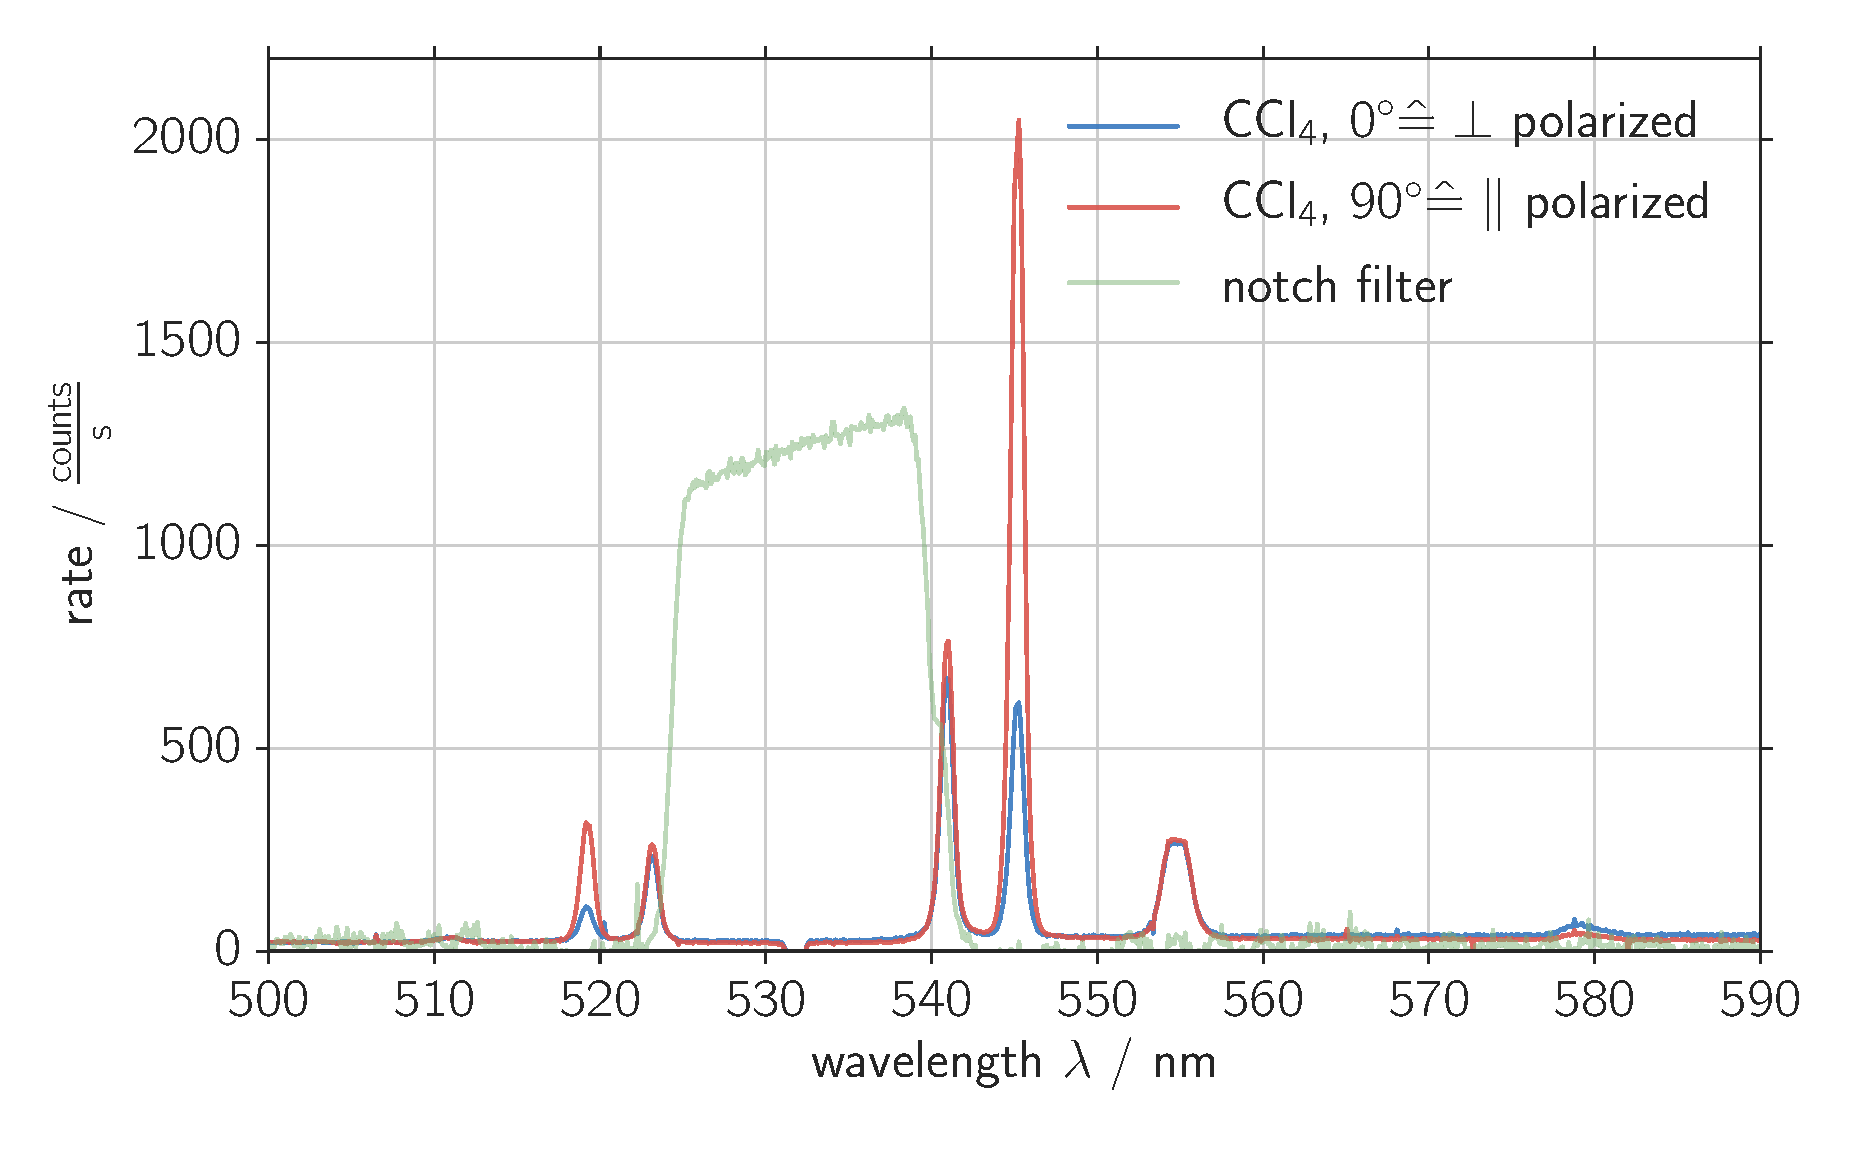
\includegraphics[width=0.8\linewidth]{analysis/figures/ccd_ccl4_spectra}
    \caption{
        Spectrum of CCl$_4$ recorded with the CCD. Three Stokes and two Anti-Stokes peaks are fitted. The two 
        small, outer peaks at 511 and 579 nm are barely visible on this scale but can been fitted well enough. 
        The notch filter blocks two more expected peaks. 
    }
    \label{fig:ccd_ccl4_spectra}
\end{figure}

\begin{table}[htpb]
    \centering
    \caption{
        Intensity and depolarization for three identified peak of the CCl$_4$ spectrum. No agreement with 
        literature data is observed.
        }
    \label{tab:ccl4_depol}
    \begin{tabular}{l c r r r r }
        \rowcolor{LightCyan} Peak N$^o$ & 
        $\Delta \nu_\text{lit} \, / \, \text{ cm}^{-1}$ & 
        $I_\perp \, / \, \frac{\text{counts}}{\text{s}}$ &
        $I_\parallel \, / \, \frac{\text{counts}}{\text{s}}$ &
        $\rho_s$  &
        $\rho_\text{lit}$\\
        \cellcolor{LightCyan}Anti-Stokes &&&&& \\
        \cellcolor{LightCyan}$1$ & $776$ & $24 \pm 2$ & $27 \pm 2$ & $0.89 \pm 0.09$ & $0.76$ \\
        \cellcolor{LightCyan}$2$ & $459$ & $123.2 \pm 1.3$ & $429.9 \pm 1.2$ & $0.287 \pm 0.003$ & $0.03$ \\
        \cellcolor{LightCyan}$3$ & $314$ & $290.8 \pm 1.3$ & $335.5 \pm 1.2$ & $0.867 \pm 0.005$ & $0.71$ \\
        \cellcolor{LightCyan}Stokes &&&&& \\
        \cellcolor{LightCyan}$4$ & $314$ & $896.6 \pm 1.4$ & $1040.5 \pm 1.3$ & $0.862 \pm 0.002$ & $0.71$ \\
        \cellcolor{LightCyan}$5$ & $459$ & $790.4 \pm 1.2$ & $2760.5 \pm 1.2$ & $0.286 \pm 0.001$ & $0.03$ \\
        \cellcolor{LightCyan}$6$ & $776$ & $752 \pm 2$ & $787 \pm 2$ & $0.956 \pm 0.003$ & $0.76$ 
    \end{tabular}
\end{table}


\subsubsection{Determining ethanol concentration}
The calculation of the ethanol requires a somewhat more sophisticated treatment of the data. 
The measurements were done with notch filter, $\lambda / 2$ plate and 1.50 A laser current, 
each one for 30 s averaged over ten times. The original data, cleared of defects, is shown 
in figure \ref{fig:ccd_ethanol_spectra}. Additionally to five Stokes peaks, one can also observe 
a broad underlying intensity distribution due to fluorescence. In order to fit the peaks and get 
their intensities, this distribution has to be subtracted. We used an algorithm that fitted a 
fourth degree polynomial to the curve, leaving out the peaks. This procedure is sketched in 
figure \ref{fig:ccd_ethanol_fluorescence} for the 60\% mixture. We don't state the polynomials as they 
are handled within the algorithm. 
The next step is shown in figure \ref{fig:ccd_ethanol_peak_fits}, where five Raman 
peaks are fitted to the rates minus the part due to fluorescence. The two overlapping peaks are fitted
simultaneously. Applying this procedure to 
the spectra a each concentration yields data about the intensity depending on the percentage of ethanol. 
Before going on, we examine the position of the peaks, similarly to the prior procedure. 
The results are shown in table \ref{tab:ccd_ethanol_peaks}. It shows good agreement with the exception 
of the second peak. This might be due to the difficulty resolving the peak due to the overlap with the 
following peak.
The linear fit of intensities over concentration is done with an orthogonal distance regression, 
since both variables have errors. The result for all five peaks is shown in figure 
\ref{fig:ccd_ethanol_intensity}. As expected, the slopes are not equal but all increasing. 
More importantly, the intersects with the corresponding peak intensities of the unknown mixture 
are all in roughly the same range. The points where linear fits and measured intensities of the original 
probe match are plotted and further listed in table \ref{tab:ccd_ethanol_peaks}. The are finally 
averaged, yielding a concentration of $(76 \pm 4)$\%. The error is estimated by the standard deviation of 
the intersects. The calculated error on each intersect turns out to be smaller than the actual deviation.
One reason is that this error ignores possible effects of systematic errors. It is further possible that 
the errors on ethanol concentration have been estimated too optimistically.
We note that the features of the original 
probe vary with respect to our prepared mixtures: While the fluorescence spectrum at 550 nm is comparable 
to the one of the 30 \% mixture, it remains much higher for larger wavelength (intersects the 60 \% mixture 
at 620 nm). Yet more striking, the Raman peaks are much higher than those of the 30 \% mixture, being of the 
same order as those of the 70 \% mixture. In our analysis, we will only use the Raman peaks and neglect the 
fluorescence part. It is not clear what the origin of these features are. We suspect effects of aging or a
contamination of the original probe. The quantitative influences are unknown and remain a mayor source of 
uncertainty. 
 
\begin{figure}[htpb]
    \centering
    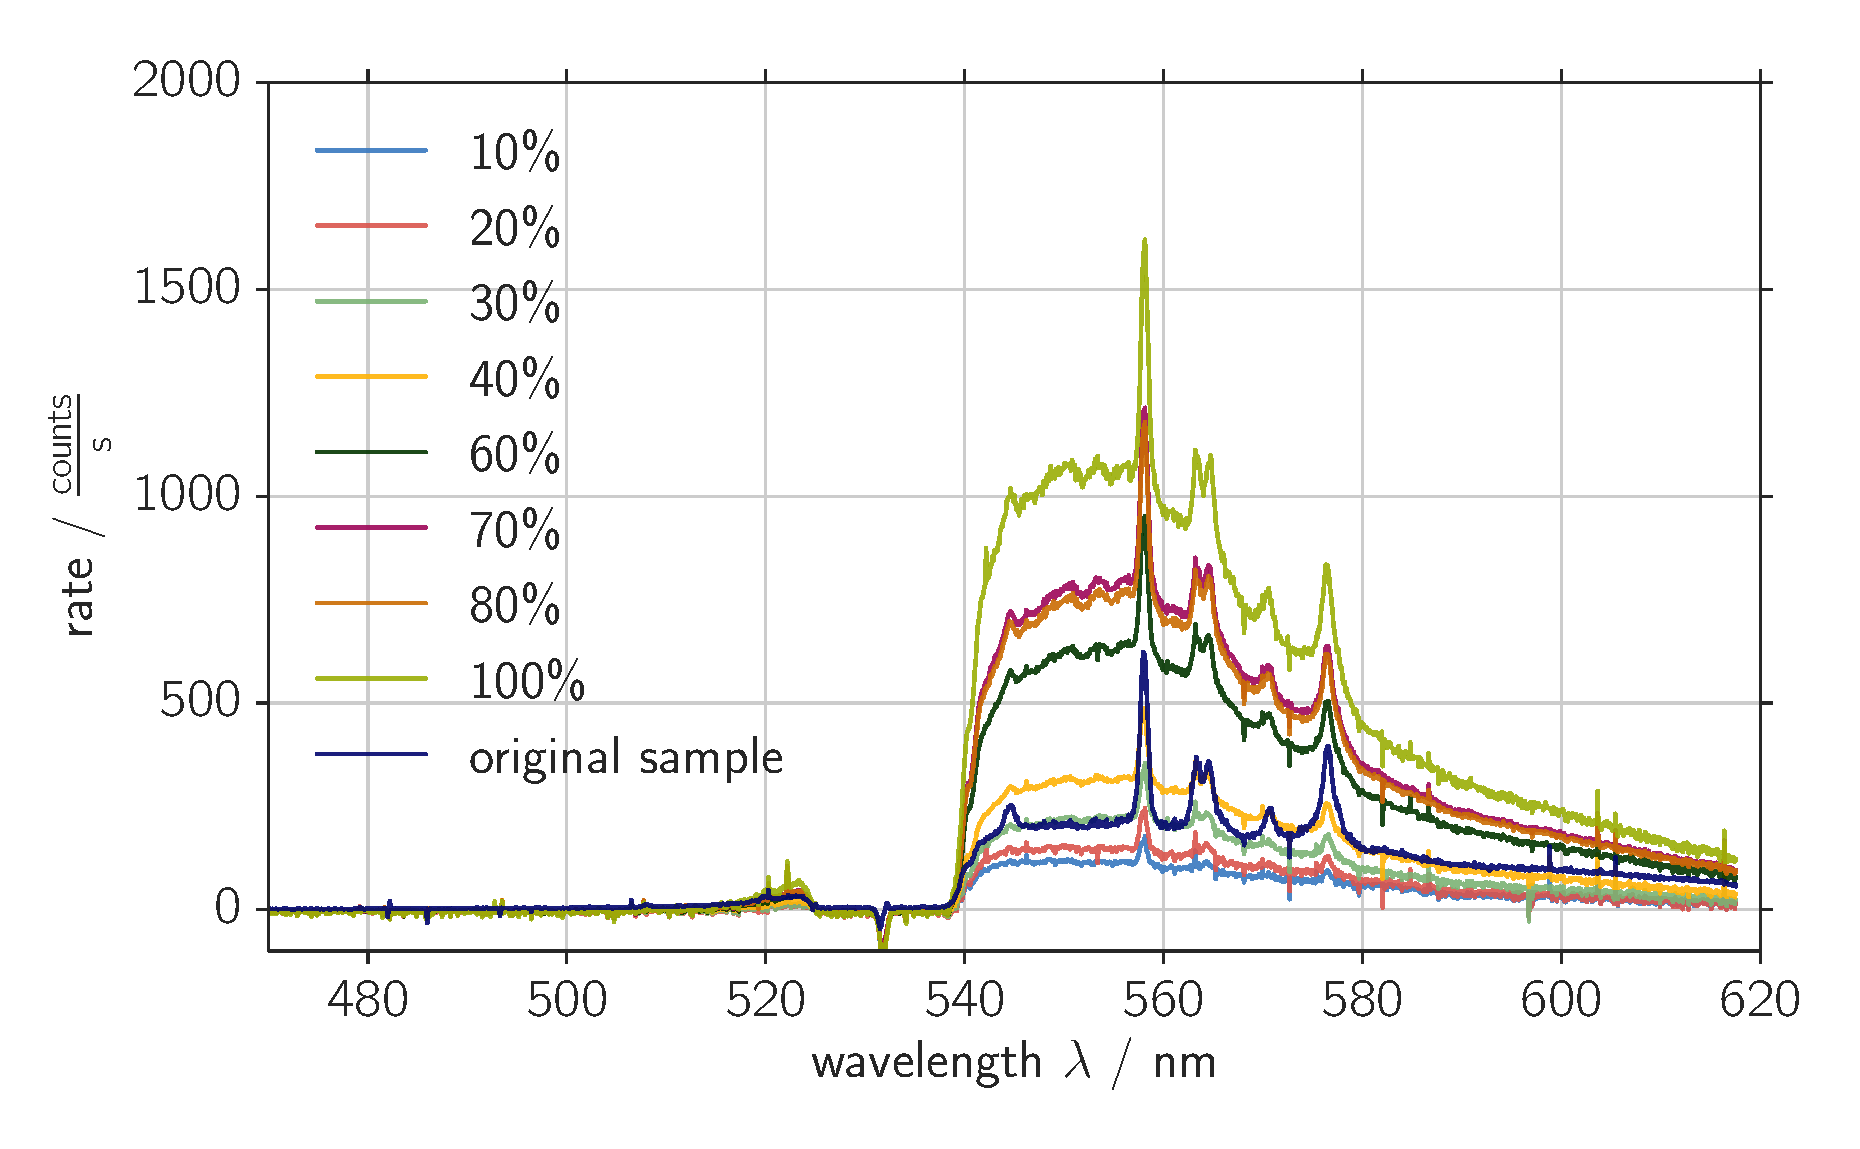
\includegraphics[width=0.8\linewidth]{analysis/figures/ccd_ethanol_spectra}
    \caption{
        Spectra of ethanol-water mix measured with the CCD spectrometer. Concentrations 
        indicate the percentage of ethanol in the mixture. The original sample has an unknown
        concentrations. Note that the fluorescence part of the original sample is much 
        lower than its Raman peaks when compared to the prepared samples. 
        }
    \label{fig:ccd_ethanol_spectra}
\end{figure}

\begin{figure}[htpb]
    \centering
    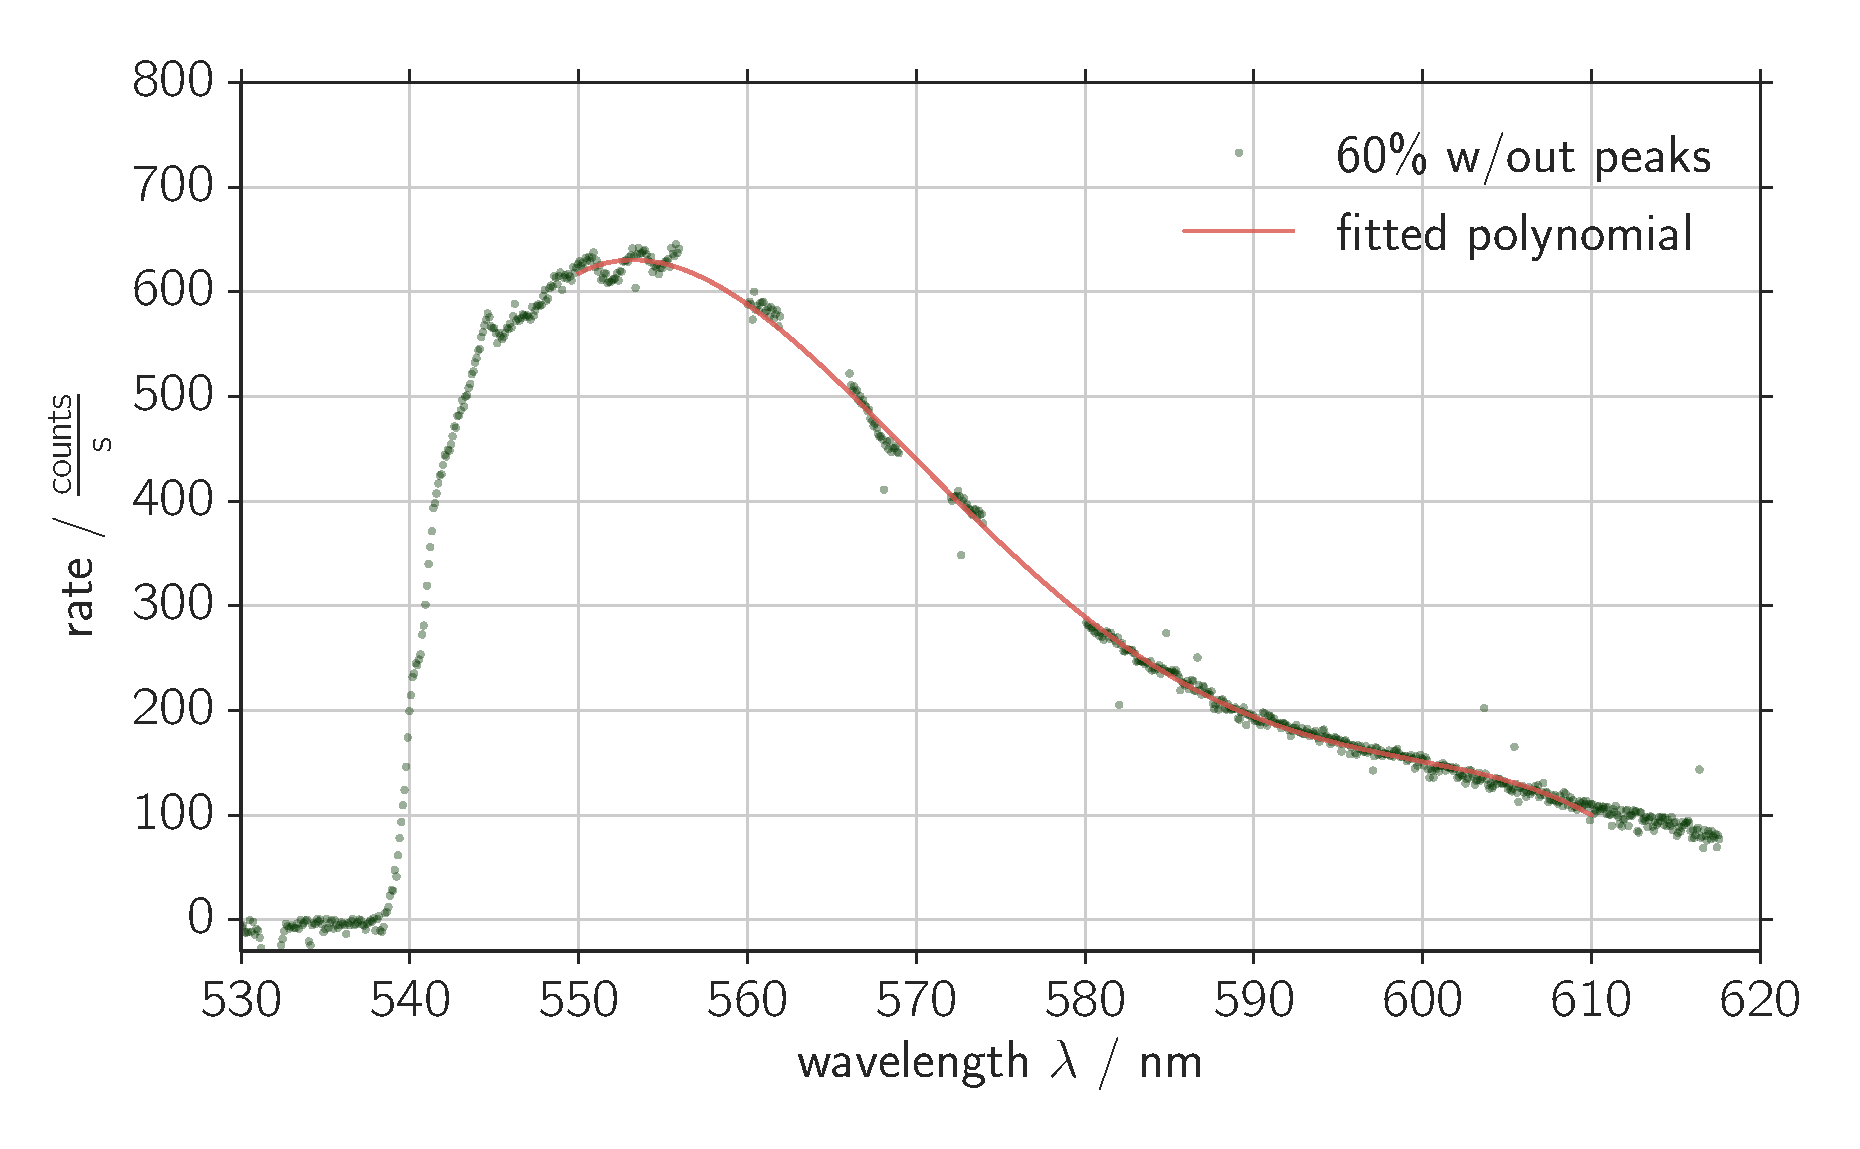
\includegraphics[width=0.8\linewidth]{analysis/figures/ccd_ethanol_fluorescence}
    \caption{
        Polynomial fit on the data of the 60\% mix, without the Raman peaks in order to subtract 
        the fluorescence part. This procedure is applied to all data. The ranges for leaving out 
        the peaks are selected manually.
        }
    \label{fig:ccd_ethanol_fluorescence}
\end{figure}

\begin{figure}[htpb]
    \centering
    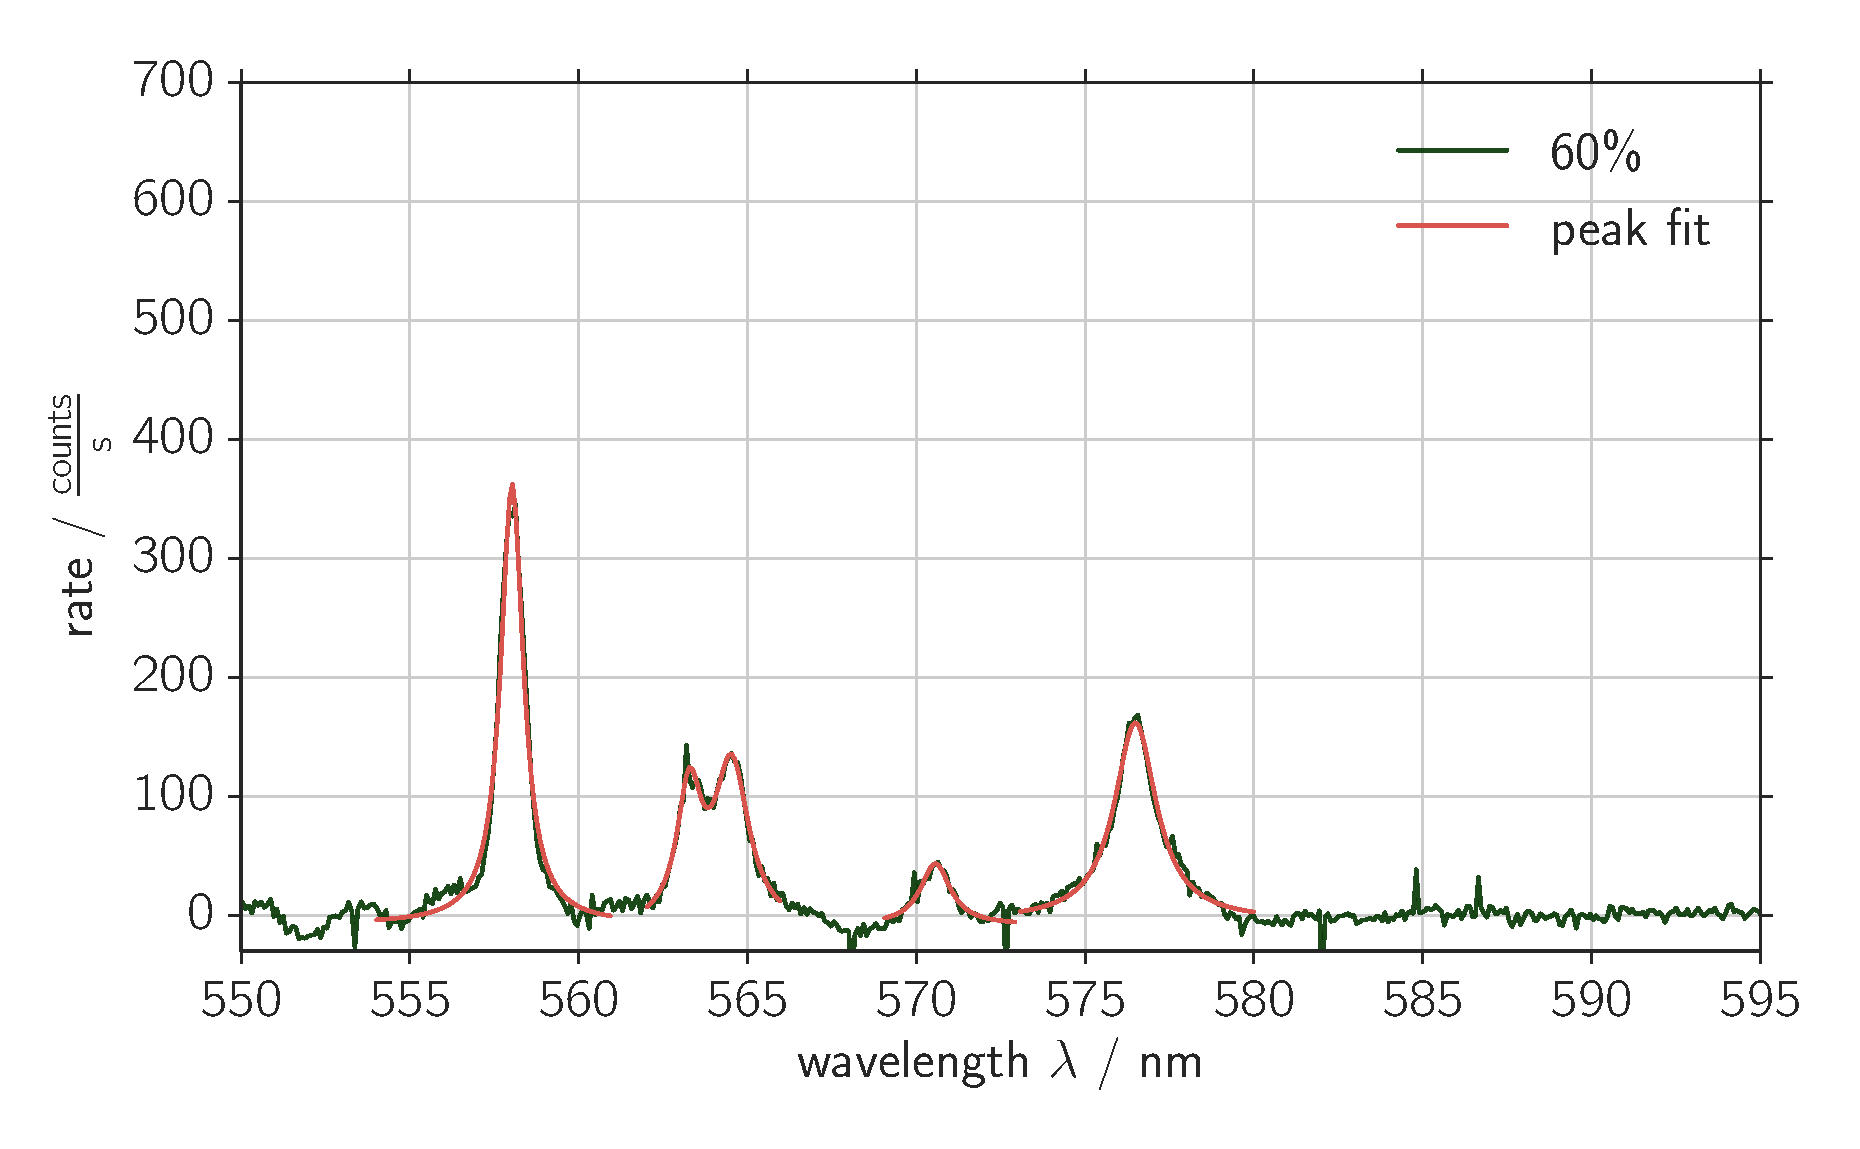
\includegraphics[width=0.8\linewidth]{analysis/figures/ccd_ethanol_peak_fits}
    \caption{
        Peak fits on the data reduced by fluorescence for the 60\% mixture. The overlapping Raman peaks 
        are fitted simultaneously. 
        }
    \label{fig:ccd_ethanol_peak_fits}
\end{figure}


\begin{table}[htpb]
    \centering
    \caption{
        Fit results of the peaks seen in the ethanol spectrum. Peaks 2 and 3 overlap. The last 
        column states the intersect with the linear fit of the intensities of each peak over 
    the ethanol concentration, see figure \ref{fig:ccd_ethanol_intensity}.
        }
    \label{tab:ccd_ethanol_peaks}
    \begin{tabular}{l r r r r}
        \rowcolor{LightCyan} Peak N$^o$ & $\lambda \, / \, \text{nm}$ &
        $\Delta \nu \, / \, \text{ cm}^{-1}$ & 
        $\Delta \nu_\text{lit} \, / \, \text{ cm}^{-1}$ &
        Intersect / \% \\
        \cellcolor{LightCyan}$1$ & $558.3 \pm 0.3$ & $880 \pm 13$ & $888$ & $72 \pm 2$  \\
        \cellcolor{LightCyan}$2$ & $563.5 \pm 0.3$ & $1047 \pm 13$ & $1028$ & $80 \pm 2$  \\
        \cellcolor{LightCyan}$3$ & $564.7 \pm 0.3$ & $1085 \pm 13$ & $1091$ & $74 \pm 2$  \\
        \cellcolor{LightCyan}$4$ & $570.8 \pm 0.3$ & $1274 \pm 13$ & $1274$ & $79 \pm 3$  \\
        \cellcolor{LightCyan}$5$ & $576.7 \pm 0.3$ & $1454 \pm 13$ & $1464$ & $73 \pm 2$  
    \end{tabular}
\end{table}

\begin{figure}[htpb]
    \centering
    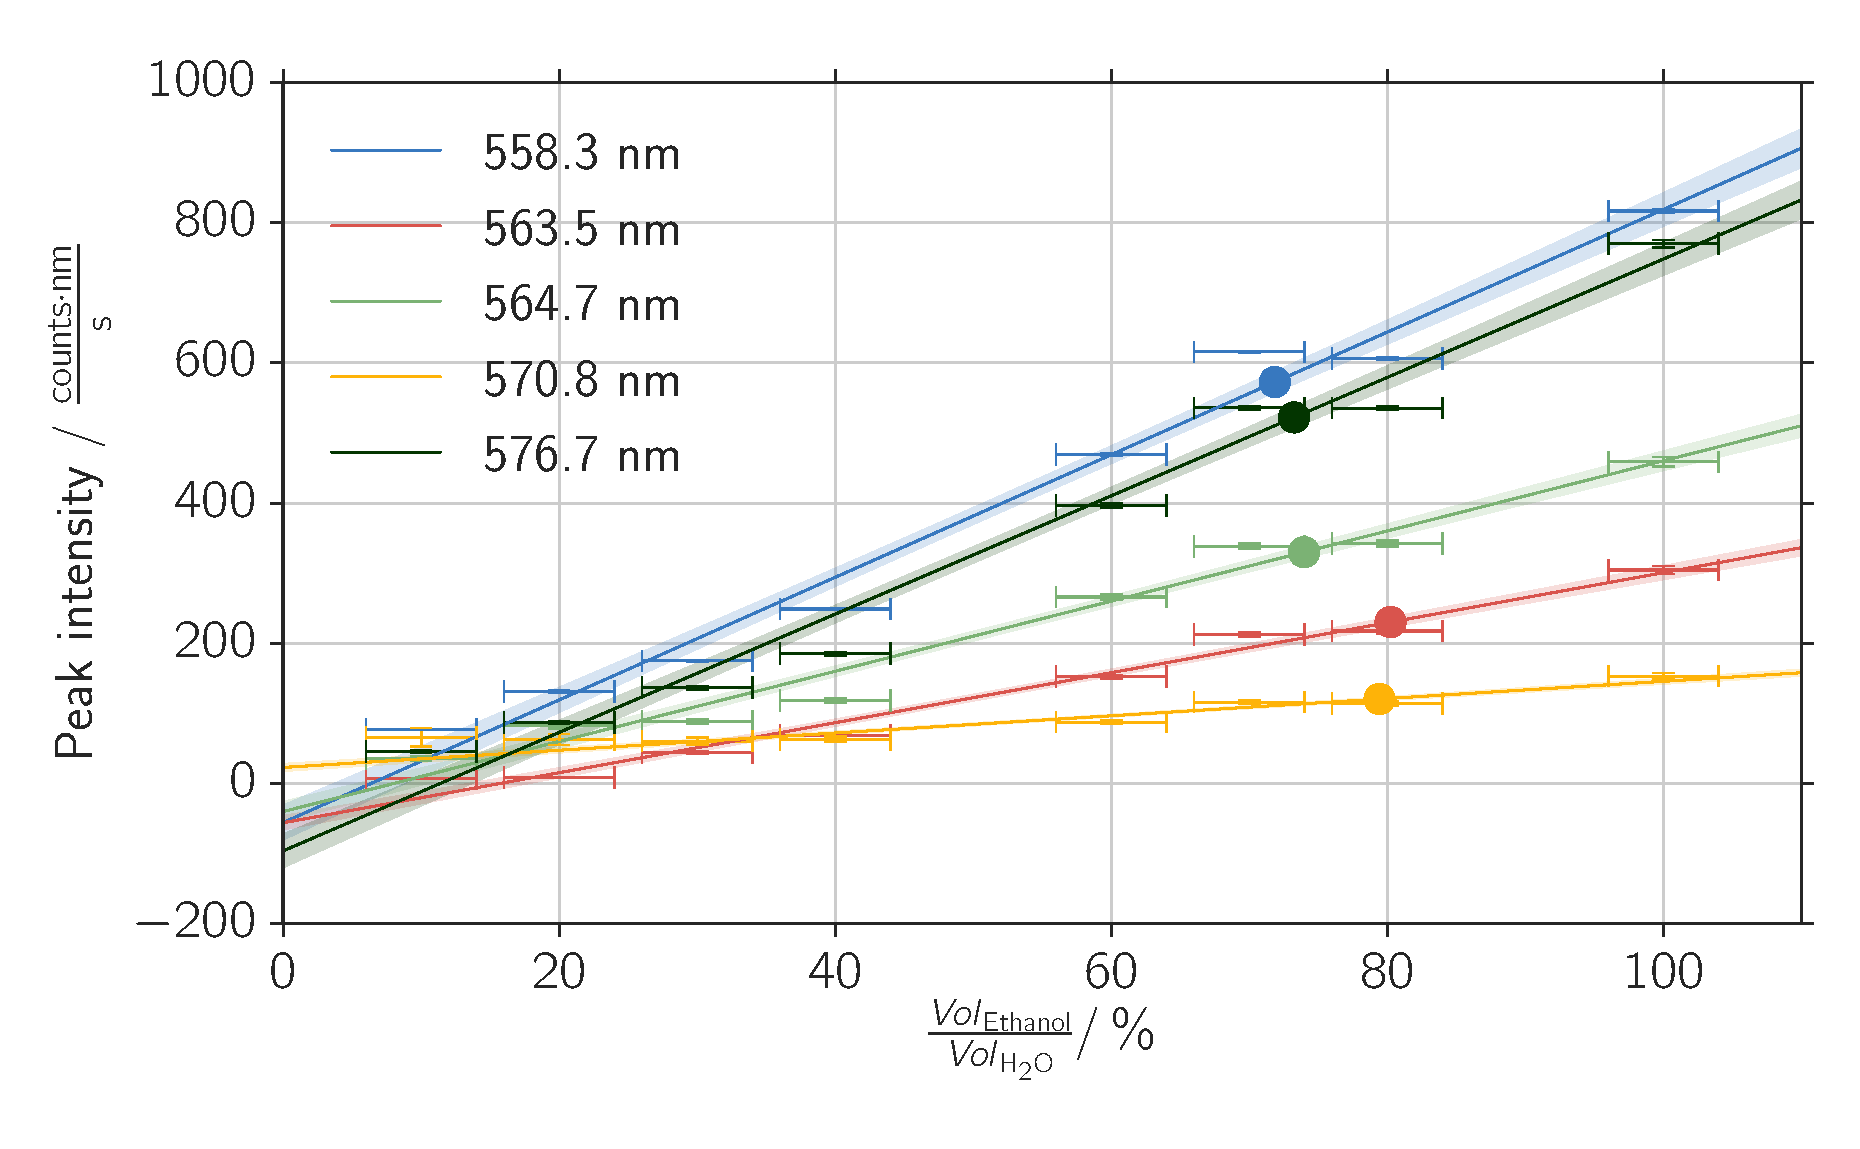
\includegraphics[width=0.8\linewidth]{analysis/figures/ccd_ethanol_intensity}
    \caption{
        Linear fits of peak intensities over ethanol concentration. The points with errorbars 
        indicate the intensities of each peak at each specific concentration. Lines 
        and shaded areas visualize the results of the linear fits. The round dots 
        correspond to the intersects where the intensity of the according peak measured 
        for the original sample matches the linear fit. For the numerical values, see table 
        \ref{tab:ccd_ethanol_peaks}
        }
    \label{fig:ccd_ethanol_intensity}
\end{figure}

\subsubsection{Temperature of sulfur sample}
The final analysis uses the dependency of relative peak intensity on the temperature as stated
in equation \eqref{eq:temp}. The procedure is straight forward: We fit a Stokes and the 
corresponding Anti-Stokes peak observable in figure \ref{fig:ccd_sulfur_spectra}. 
The peaks are found to be centered at $545.6 \pm 0.3$ nm 
and $518.8 \pm 0.3$ nm, which corresponds to a distance to the laser peak of $463 \pm 13$ and 
$482 \pm 14$ cm$^{-1}$. We did not find literature values for a direct comparison. 
The intensities are taken directly from the fit. They and the ratio of Anti-Stokes to Stokes
intensity are listed in table \ref{tab:sulfur_intensity} and plotted in figure 
\ref{fig:ccd_temp_rate}. The value needed for our analysis 
is the mean of the ratios. It is given by 
\begin{equation*}
    \overline{\frac{I_\text{Anti-Stokes}}{I_\text{Stokes}}} = 0.129 \pm 0.007 \, .
\end{equation*}
We use this value to calculate the temperature by inverting the previously stated relation, 
thus 
\begin{equation}
    T = \frac{-h \Delta \nu}{
        k_b \cdot \ln \left(
            \frac{I_\text{Anti-Stokes}}{I_\text{Stokes}} \cdot \left(\frac{\nu_\text{laser} - 
            \Delta \nu}{\nu_\text{laser} + \Delta \nu}\right)^4 
    \right)} \, .
\end{equation}
Our result is 
\begin{equation}
    T = (29 \pm 8) ^\circ C \, .
\end{equation}
Since room temperature was measured with $T_\text{room} = (20.3 \pm 0.3) ^\circ C$, this is too high. 
One could argue that the temperature of the sample rose due to the incident laser radiation. 
We are, however, rather skeptical towards this position and highlight the various possible 
systematic errors which could induce the observed higher temperature. 
One example is the sample itself: The sample inside a glass container had to be positioned 
by hand at an arbitrary angle, as long as Bragg reflection would not enter the Beam path 
(i.~e. not at 45$^\circ$). We chose an angle such that Bragg reflection occurred at about 
$60^\circ$. In any case, the failure of this 
measurement has been reported various times before (see e.~g. \cite{wiss}). 

\begin{figure}[htpb]
    \centering
    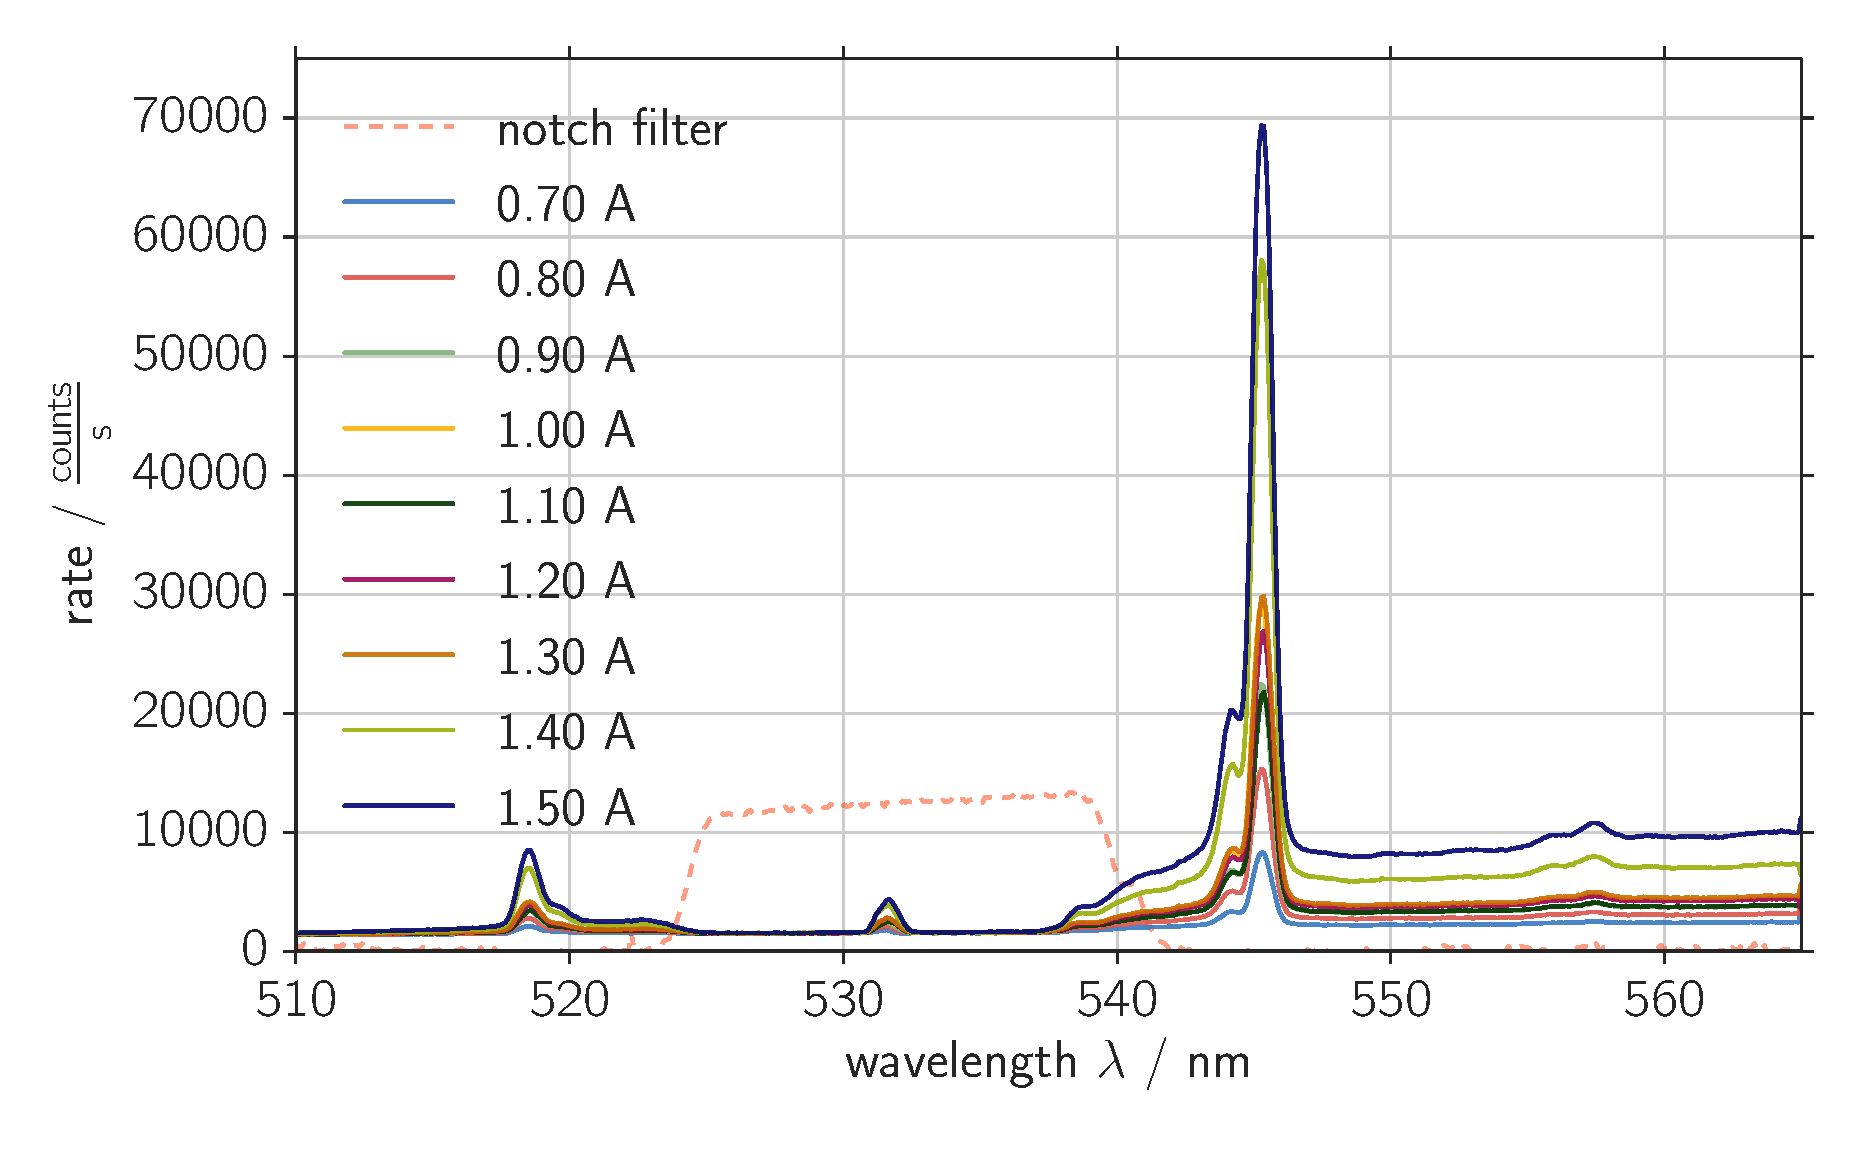
\includegraphics[width=0.8\linewidth]{analysis/figures/ccd_sulfur_spectra}
    \caption{
        Raman spectra of the sulfur sample measured with the CCD spectrometer for different 
        laser currents (values shown in the legend in Ampere). The notch filter's 
        effect is plotted for convenience. One can observe a strong dependence of peak intensity 
        on the applied laser current. The intensity ratio, however, is expected to be independent 
        thereof. 
        }
    \label{fig:ccd_sulfur_spectra}
\end{figure}


\begin{table}[htpb]
    \centering
    \caption{
        Intensities and ratio for Stokes and Anti-Stokes peak of sulfur spectrum.
        }
    \label{tab:sulfur_intensity}
    \begin{tabular}{l r r r}
        \rowcolor{LightCyan}$I_\text{laser} \, / \, \text{A}$ & 
        $I_\text{Stokes} \, / \, \frac{\text{counts}}{\text{s}}$ &
        $I_\text{Anti-Stokes} \, / \, \frac{\text{counts}}{\text{s}}$ &
        $\frac{I_\text{Anti-Stokes}}{I_\text{Stokes}}$ \\
        \cellcolor{LightCyan}$0.70$ A & $7462 \pm 6$ & $1096 \pm 5$ & $0.1468 \pm 0.0006$   \\
        \cellcolor{LightCyan}$0.80$ A & $15187 \pm 7$ & $2004 \pm 4$ & $0.1320 \pm 0.0003$   \\
        \cellcolor{LightCyan}$0.90$ A & $22940 \pm 8$ & $2952 \pm 4$ & $0.1287 \pm 0.0002$   \\
        \cellcolor{LightCyan}$1.00$ A & $30256 \pm 8$ & $3834 \pm 4$ & $0.1267 \pm 0.0002$   \\
        \cellcolor{LightCyan}$1.10$ A & $22607 \pm 7$ & $2866 \pm 5$ & $0.1268 \pm 0.0002$   \\
        \cellcolor{LightCyan}$1.20$ A & $28225 \pm 8$ & $3552 \pm 5$ & $0.1259 \pm 0.0002$   \\
        \cellcolor{LightCyan}$1.30$ A & $31637 \pm 8$ & $3939 \pm 5$ & $0.1245 \pm 0.0002$   \\
        \cellcolor{LightCyan}$1.40$ A & $62397 \pm 9$ & $7582 \pm 5$ & $0.12151 \pm 0.00008$   \\
        \cellcolor{LightCyan}$1.50$ A & $77655 \pm 10$ & $9649 \pm 5$ & $0.12425 \pm 0.00007$   
    \end{tabular}
\end{table}

\begin{figure}[htpb]
    \centering
    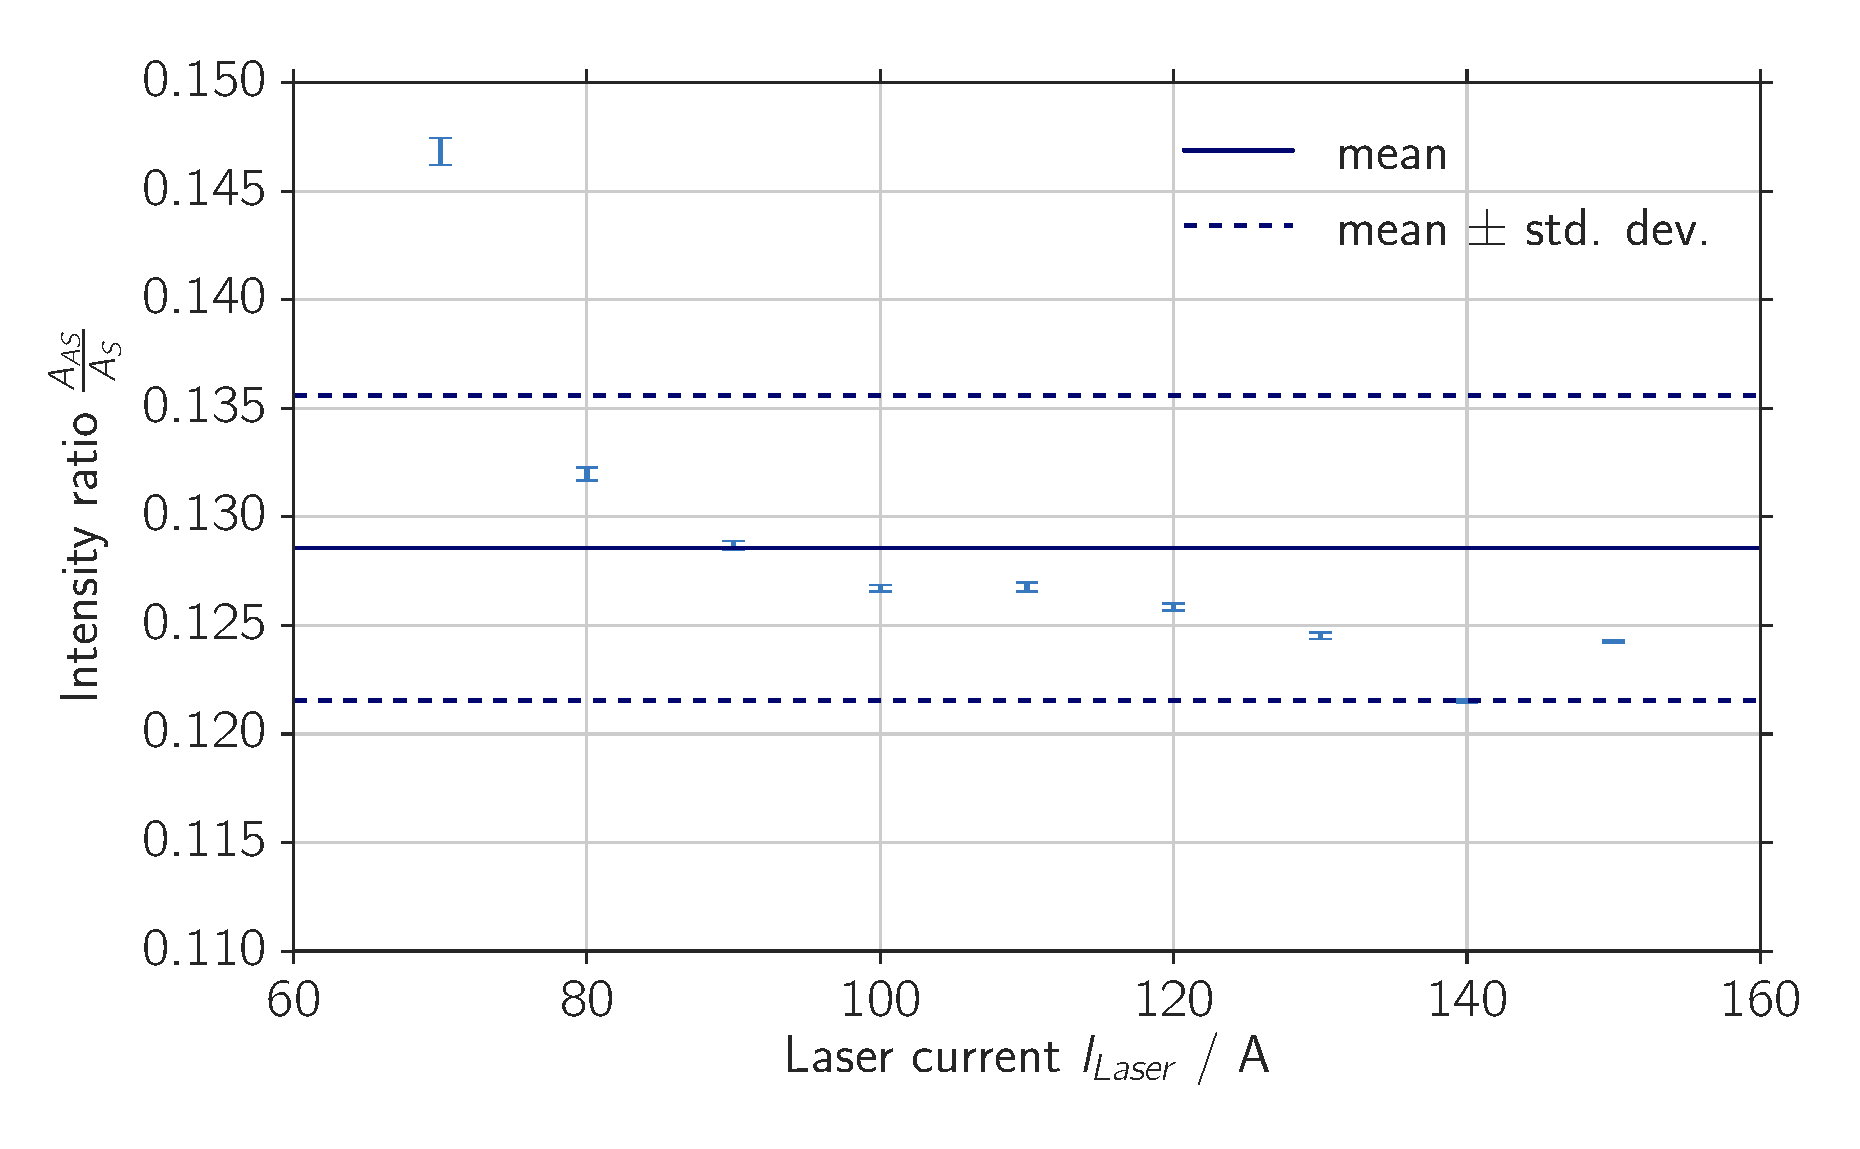
\includegraphics[width=0.8\linewidth]{analysis/figures/ccd_temp_rate}
    \caption{
        Ratio of intensities of Stokes and Anti-Stokes peaks for different laser currents. 
        The expectation of a constant value (for constant temperature) is not met for the 
        calculated standard deviations. These do not include systematical errors, however. 
        }
    \label{fig:ccd_temp_rate}
\end{figure}

